% LaTEX source code
% Last modified November 1st, 2005
% Steve Miller
% note that the percent sign comments out the rest of the line
% first, we set a document class. often use 12pt characters, though
% sometimes people do 11 or 10. you can do report or article, both similar
%\documentclass[12pt,letterpaper]{article}
\documentclass[12pt,reqno]{amsart}
\linespread{1}
\addtolength{\textwidth}{2cm} \addtolength{\hoffset}{-1cm}
\addtolength{\marginparwidth}{-1cm} \addtolength{\textheight}{2cm}
\addtolength{\voffset}{-1cm}
% below are some packages that are needed for certain symbols, graphics, colors.
% safest to just include these.
\usepackage{times}
\usepackage[T1]{fontenc}
\usepackage{mathrsfs}
\usepackage{latexsym}
\usepackage[dvips]{graphics}
\usepackage{epsfig}
\usepackage{hyperref, amsmath, amsthm, amsfonts, amscd, flafter,epsf}
\usepackage{amsmath,amsfonts,amsthm,amssymb,amscd}
\input amssym.def
\input amssym.tex
\usepackage{color}
\usepackage{enumerate}
\usepackage{hyperref}
\usepackage{url}
\usepackage{floatrow}
\usepackage{caption}
\usepackage{subcaption}
\usepackage{capt-of}
\usepackage{physics}
\newcommand{\todo}[1]{\textcolor{red}{\textbf{(#1)}}}

    %=======================================================

    %   THIS IS WHERE YOU PUT SHORTCUT DEFINITIONS

    %========================================================

% Note that we use a percent sign to comment out a line

% below are shortcut commands

%%%%%%%%%%%%%%%%%%%%%%%%%%%%%%%%%%%%%%%%%%%%%%%

% below are shortcuts for equation, eqnarray,

% itemize and enumerate environments

\newcommand\be{\begin{equation}}
\newcommand\ee{\end{equation}}
\newcommand\bea{\begin{eqnarray}}
\newcommand\eea{\end{eqnarray}}
\newcommand\bi{\begin{itemize}}
\newcommand\ei{\end{itemize}}
\newcommand\ben{\begin{enumerate}}
\newcommand\een{\end{enumerate}}
\newcommand{\ncr}[2]{\left({#1 \atop #2}\right)}
%%%%%%%%%%%%%%%%%%%%%%%%%%%%%%%%%%%%%%%%%%%%%%%%

% Theorem / Lemmas et cetera

\newtheorem{thm}{Theorem}[section]
\newtheorem{conj}[thm]{Conjecture}
\newtheorem{cor}[thm]{Corollary}
\newtheorem{lem}[thm]{Lemma}
\newtheorem{prop}[thm]{Proposition}
\newtheorem{exa}[thm]{Example}
\newtheorem{defi}[thm]{Definition}
\newtheorem{exe}[thm]{Exercise}
\newtheorem{rek}[thm]{Remark}
\newtheorem{que}[thm]{Question}
\newtheorem{prob}[thm]{Problem}
\newtheorem{cla}[thm]{Claim}
\newtheorem{defis}[thm]{Definitions}
\newtheorem{res}[thm]{Result}
\newtheorem{calc}[thm]{Calculation}
%%%%%%%%%%%%%%%%%%%%%%%%%%%%%%%%%%%%%%%%%

% shortcuts to environments

% this allows you to do textboldface: simply type \tbf{what you want in bold}

\newcommand{\tbf}[1]{\textbf{#1}}

%%%%%%%%%%%%%%%%%%%%%%%%%%%%%%%%%%%%%%%%%%%%%%%%%%

% shortcut to twocase and threecase definitions

\newcommand{\twocase}[5]{#1 \begin{cases} #2 & \text{#3}\\ #4
&\text{#5} \end{cases}   }
\newcommand{\threecase}[7]{#1 \begin{cases} #2 &
\text{#3}\\ #4 &\text{#5}\\ #6 &\text{#7} \end{cases}   }
%%%%%%%%%%%%%%%%%%%%%%%%%%%%%%%%%%%%%%%%%

%Blackboard Letters

\newcommand{\R}{\ensuremath{\mathbb{R}}}
\newcommand{\C}{\ensuremath{\mathbb{C}}}
\newcommand{\Z}{\ensuremath{\mathbb{Z}}}
\newcommand{\Q}{\mathbb{Q}}
\newcommand{\N}{\mathbb{N}}
\newcommand{\F}{\mathbb{F}}
\newcommand{\W}{\mathbb{W}}
\newcommand{\Qoft}{\mathbb{Q}(t)}  %use in linux
\newcommand{\soln}{\noindent \textbf{Solution:}\ }

%%%%%%%%%%%%%%%%%%%%%%%%%%%%%%%%%%%%%%%%%

% Finite Fields and Groups

\newcommand{\Fp}{ \F_p }
%%%%%%%%%%%%%%%%%%%%%%%%%%%%%%%%%%%%%%%%%

% Fractions

\newcommand{\foh}{\frac{1}{2}}  %onehalf
\newcommand{\fot}{\frac{1}{3}}
\newcommand{\fof}{\frac{1}{4}}

%%%%%%%%%%%%%%%%%%%%%%%%%%%%%%%%%%%%%%%%%

% Legendre Symbols

\newcommand{\js}[1]{ { \underline{#1} \choose p} }

%%%%%%%%%%%%%%%%%%%%%%%%%%%%%%%%%%%%%%%%%

% matrix shortcuts

\newcommand{\mattwo}[4]
{\left(\begin{array}{cc}
                        #1  & #2   \\
                        #3 &  #4
                          \end{array}\right) }
\newcommand{\matthree}[9]
{\left(\begin{array}{ccc}
                        #1  & #2 & #3  \\
                        #4 &  #5 & #6 \\
                        #7 &  #8 & #9
                          \end{array}\right) }
\newcommand{\dettwo}[4]
{\left|\begin{array}{cc}
                        #1  & #2   \\
                        #3 &  #4
                          \end{array}\right| }
\newcommand{\detthree}[9]
{\left|\begin{array}{ccc}
                        #1  & #2 & #3  \\
                        #4 &  #5 & #6 \\
                        #7 &  #8 & #9
                          \end{array}\right| }
%%%%%%%%%%%%%%%%%%%%%%%%%%%%%%%%%%%%%%%%%

% greek letter shortcuts

\newcommand{\ga}{\alpha}                  %gives you a greek alpha
\newcommand{\gb}{\beta}
\newcommand{\gep}{\epsilon}
%%%%%%%%%%%%%%%%%%%%%%%%%%%%%%%%%%%%%%%%%

% general functions

\newcommand{\notdiv}{\nmid}               % gives the not divide symbol
\newcommand{\burl}[1]{\textcolor{blue}{\url{#1}}}

%%%%%%%%%%%%%%%%%%%%%%%%%%%%%%%%%%%%%%%%%%%

% the following makes the numbering start with 1 in each section;

% if you want the equations numbered 1 to N (without caring about

% what section you are in, comment out the following line.

\numberwithin{equation}{section}

%\textwidth= 6in

%\evensidemargin=37pt

%\oddsidemargin=0pt

\begin{document}



\title{Hexane Water Results Log}
\author{Kirk Swanson}
\email{swansonk1@uchicago.edu}
\address{Institute for Molecular Engineering, University of Chicago, 5640 S Ellis Ave, Chicago, IL 60637}
%\keywords{path integral molecular dynamics, path integral monte carlo, metropolis algorithm}
\date{\today}




\maketitle

%%%%%%%%%%%%%%%%%%%%%%%%%%%%%%%%%%%%%%%%%%%%%%%%%%%%%%%%%%%%%%%%%%%%%%%%%%%%%%%%%%%%%%%%%%%%%%%%%%%%%%%%%%%%%%%%%%%%%%%%%%%%%%

\normalsize

%%%%%%%%%%%%%%%%%%%%%%%%%%%%%%%%%%%%%%%%%%%%%%%%%%%%%%%%%%%%%%%%%%%%%%%%%%%%%%%%%%%%%%%%%%%%%%%%%%%%%%%%%%%%%%%%%%%%%%%%%%%%%%

\section{1/8/2018}
\begin{enumerate}
\item Ran a simulation of the hexane-water interface using LAMMPS.  Set up for 1M time steps, but only got through 745,200 due to time limit of 24 hrs.  
\item Ran a simulation of the hexane-water interface in DASH, using the python script "interface.py" in the dash-work/interface folder.  The run was for 4,000,000 time steps, printing a configuration every 50,000 steps.  Below are snapshots of the 0th timestep and the 3,950,000 time step.    

\begin{figure}[H]
\centering
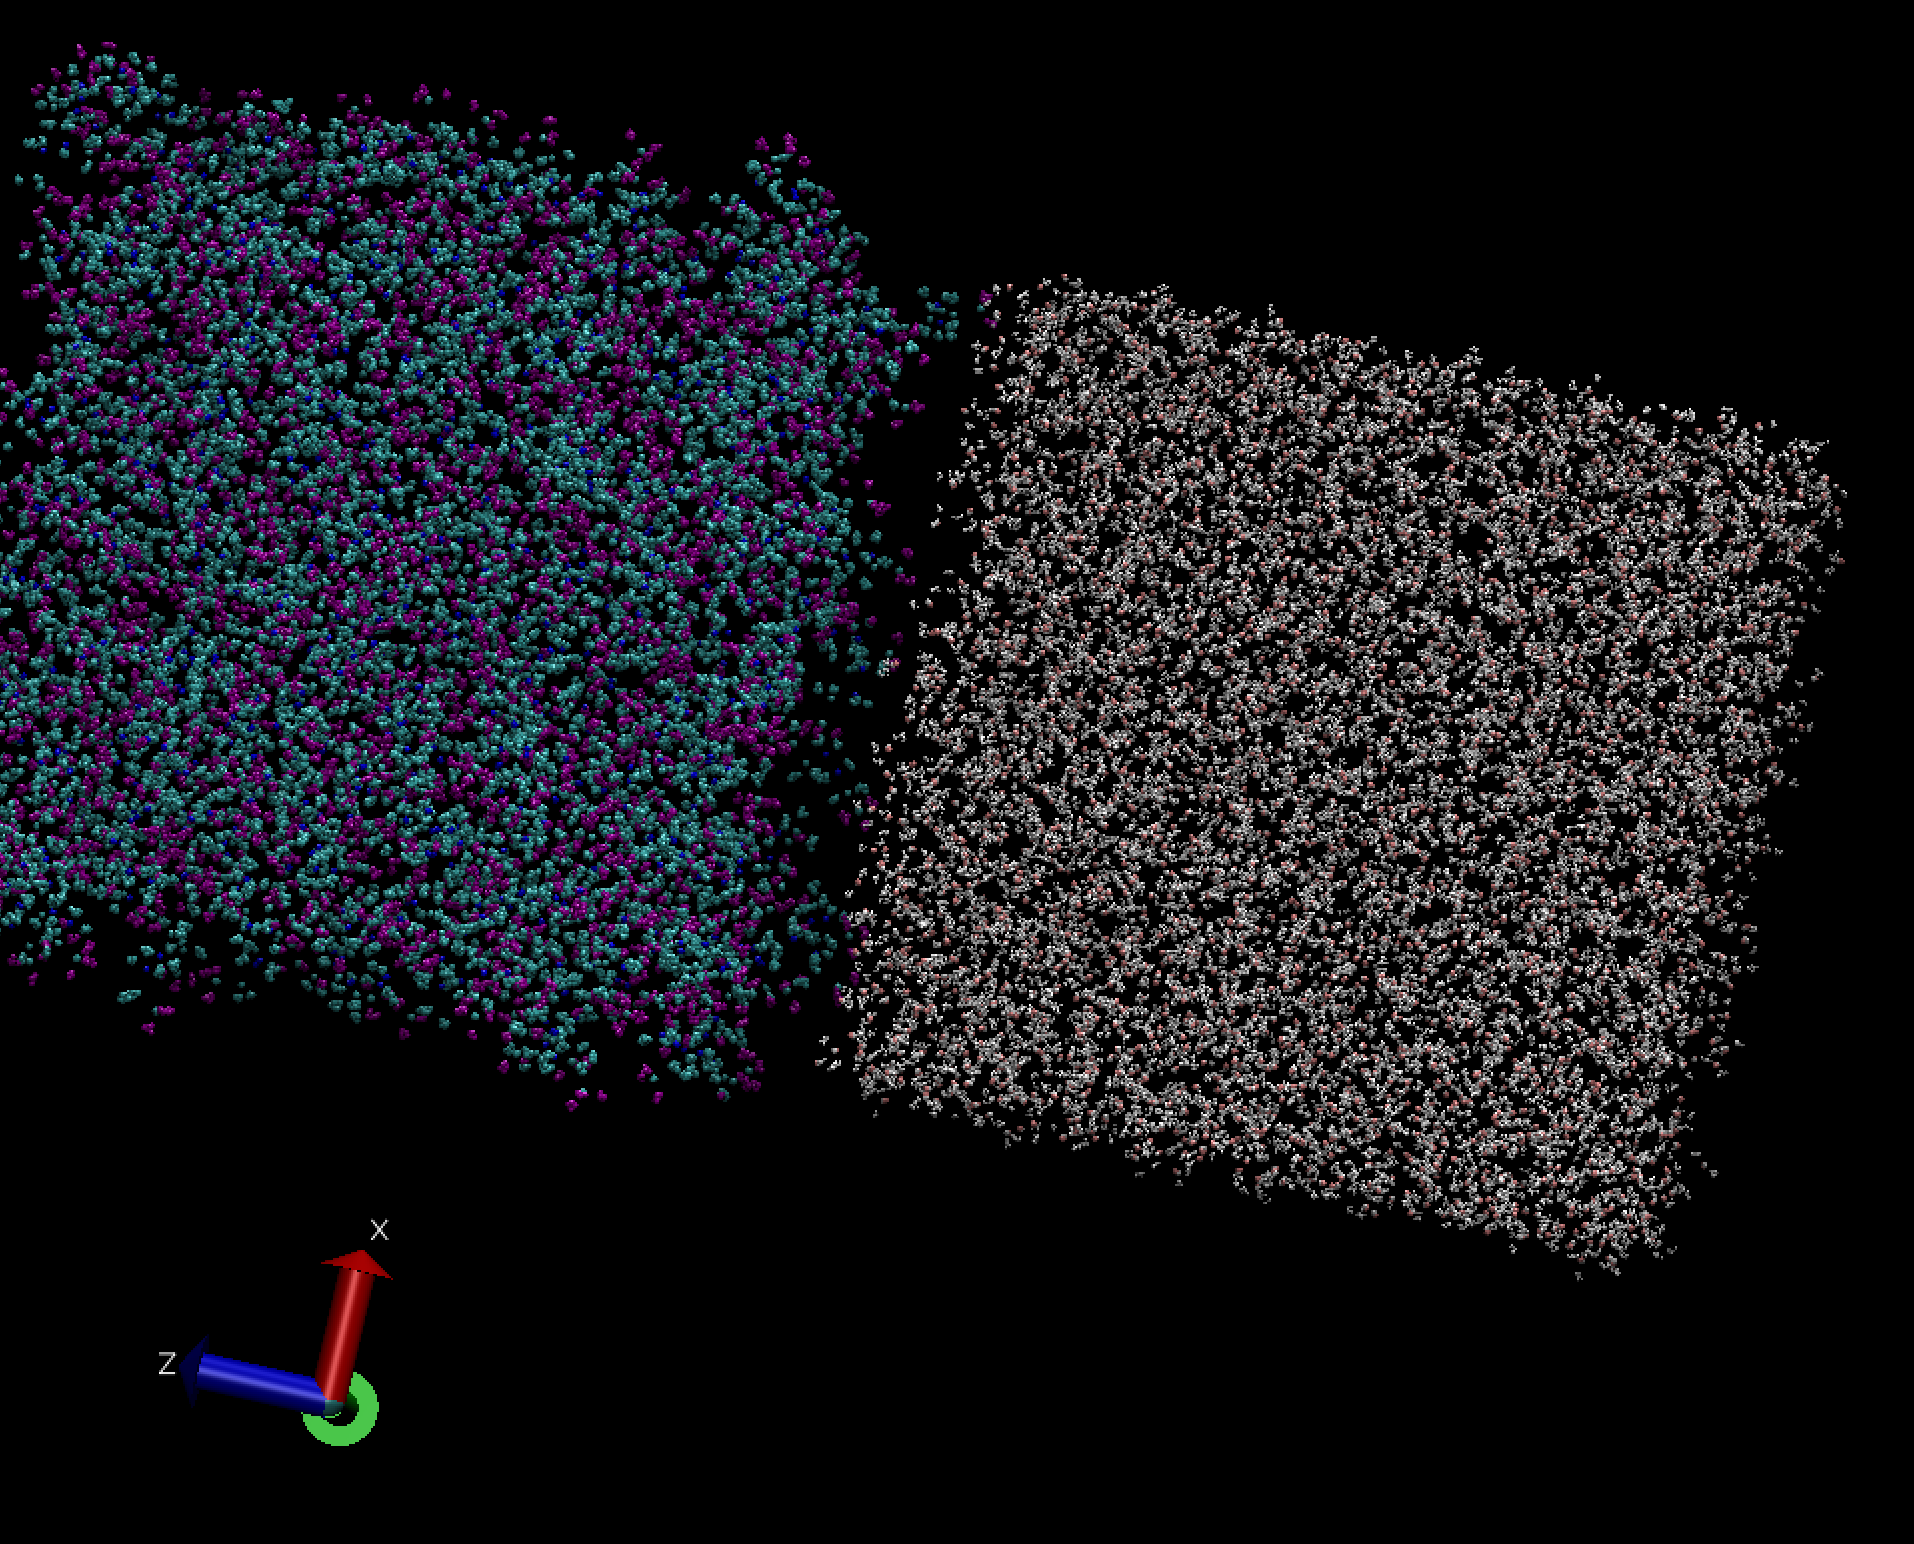
\includegraphics[scale=0.4]{dash_taffi-tip4pF_8beads_0}
\caption{DASH simulation of the TAFFI - q-TIP4P/F interface.  Arithmetic mixing, 4,000,000 time steps.  This is the 0th timestep.}
\end{figure}

\begin{figure}[H]
\centering
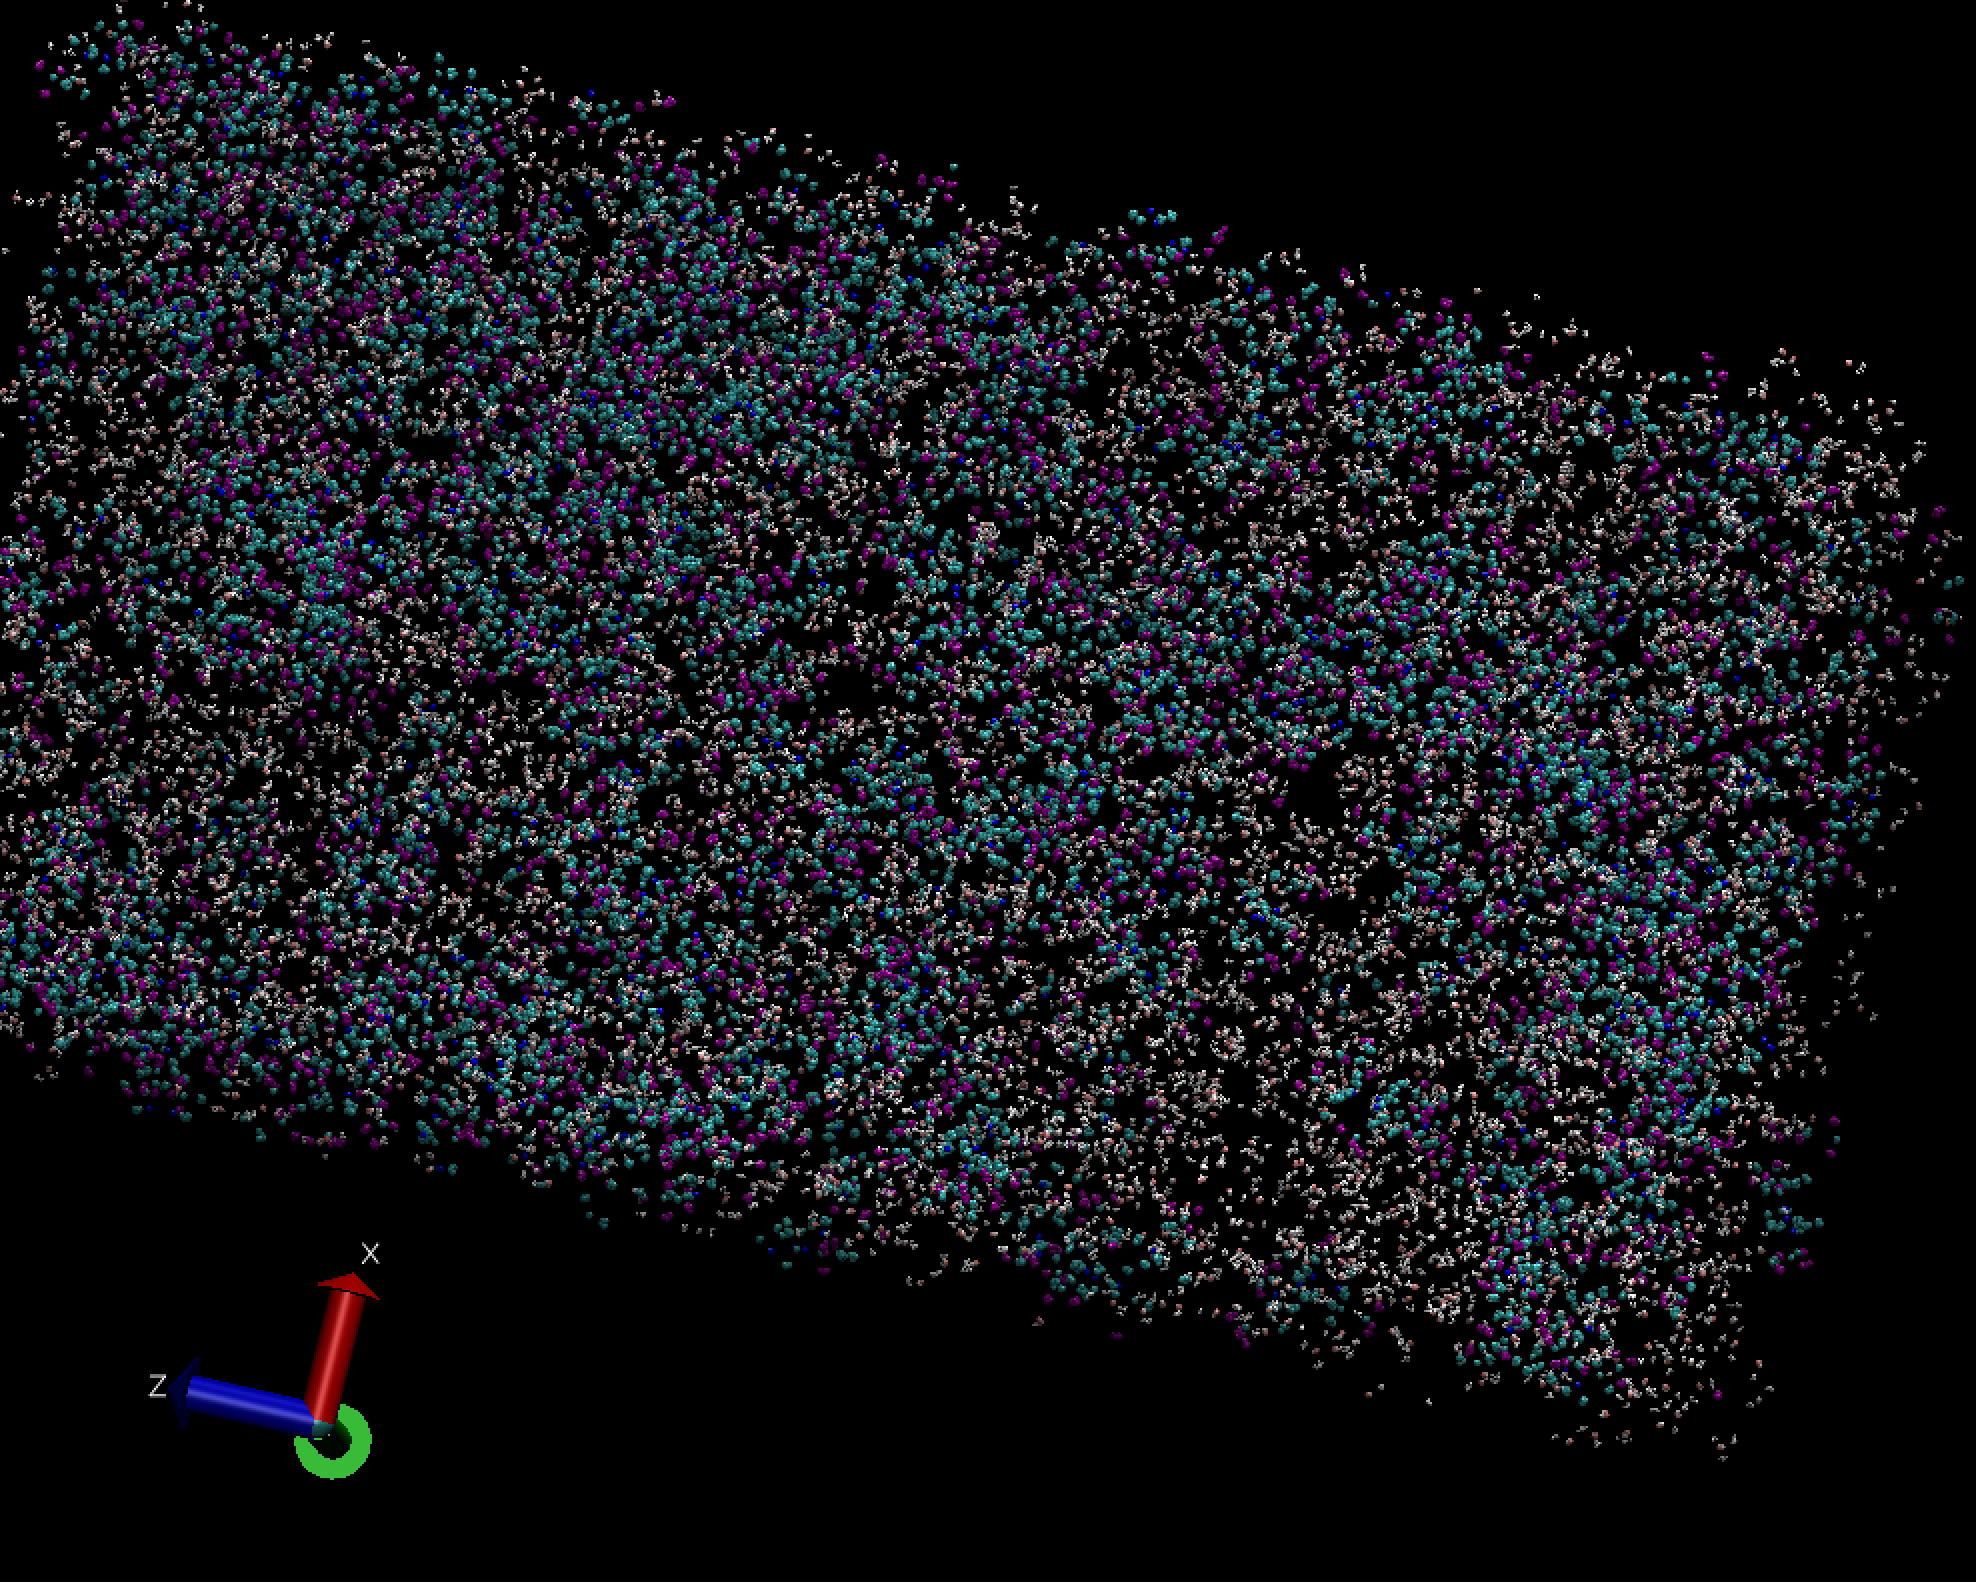
\includegraphics[scale=0.4]{dash_taffi-tip4pF_8beads_3950000}
\caption{DASH simulation of the TAFFI - q-TIP4P/F interface.  Arithmetic mixing, 4,000,000 time steps.  This is the 3,950,000th timestep.}
\end{figure}

\item This is in stark contrast to the amount of mixing that we observed in OPLS + TIP4P/2005 in LAMMPS, which was the appropriate amount of mixing, i.e., very little mixing.  So, there are several possible things going on here.  One is that there is an error in the code.  Another is that there is an error in DASH.  And third is that there is a problem with the interaction parameters between the two force fields.  So, here are the following tests that we are going to run to narrow down the problem:
\subitem Run TAFFI + TIP4P/F in LAMMPS using arithmetic, geometric, and Waldman-Hagler mixing rules and using both TAFFI and OPLS parameters for hexane 
\subitem Run TAFFI + TIP4P/F in DASH using geometric and Waldman-Hagler mixing rules using both TAFFI and OPLS parameters and using 1 bead versus 8 beads
\subitem Run OPLS + TIP4P/F in DASH using geometric mixing rules and using 1 bead versus 8 beads
\subitem Check for any errors in the DASH input scripts
\subitem TAFFI + TIP4P/F in DASH using on bead

\item So, the first step we are going to take is to run TAFFI + q-TIP4P/F in LAMMPS using arithmetic mixing rules.  Let's first take a look at the simulation of TAFFI + TIP4P/2005 and see what that snapshot looks like.  At timestep zero:

\begin{figure}[H]
\centering
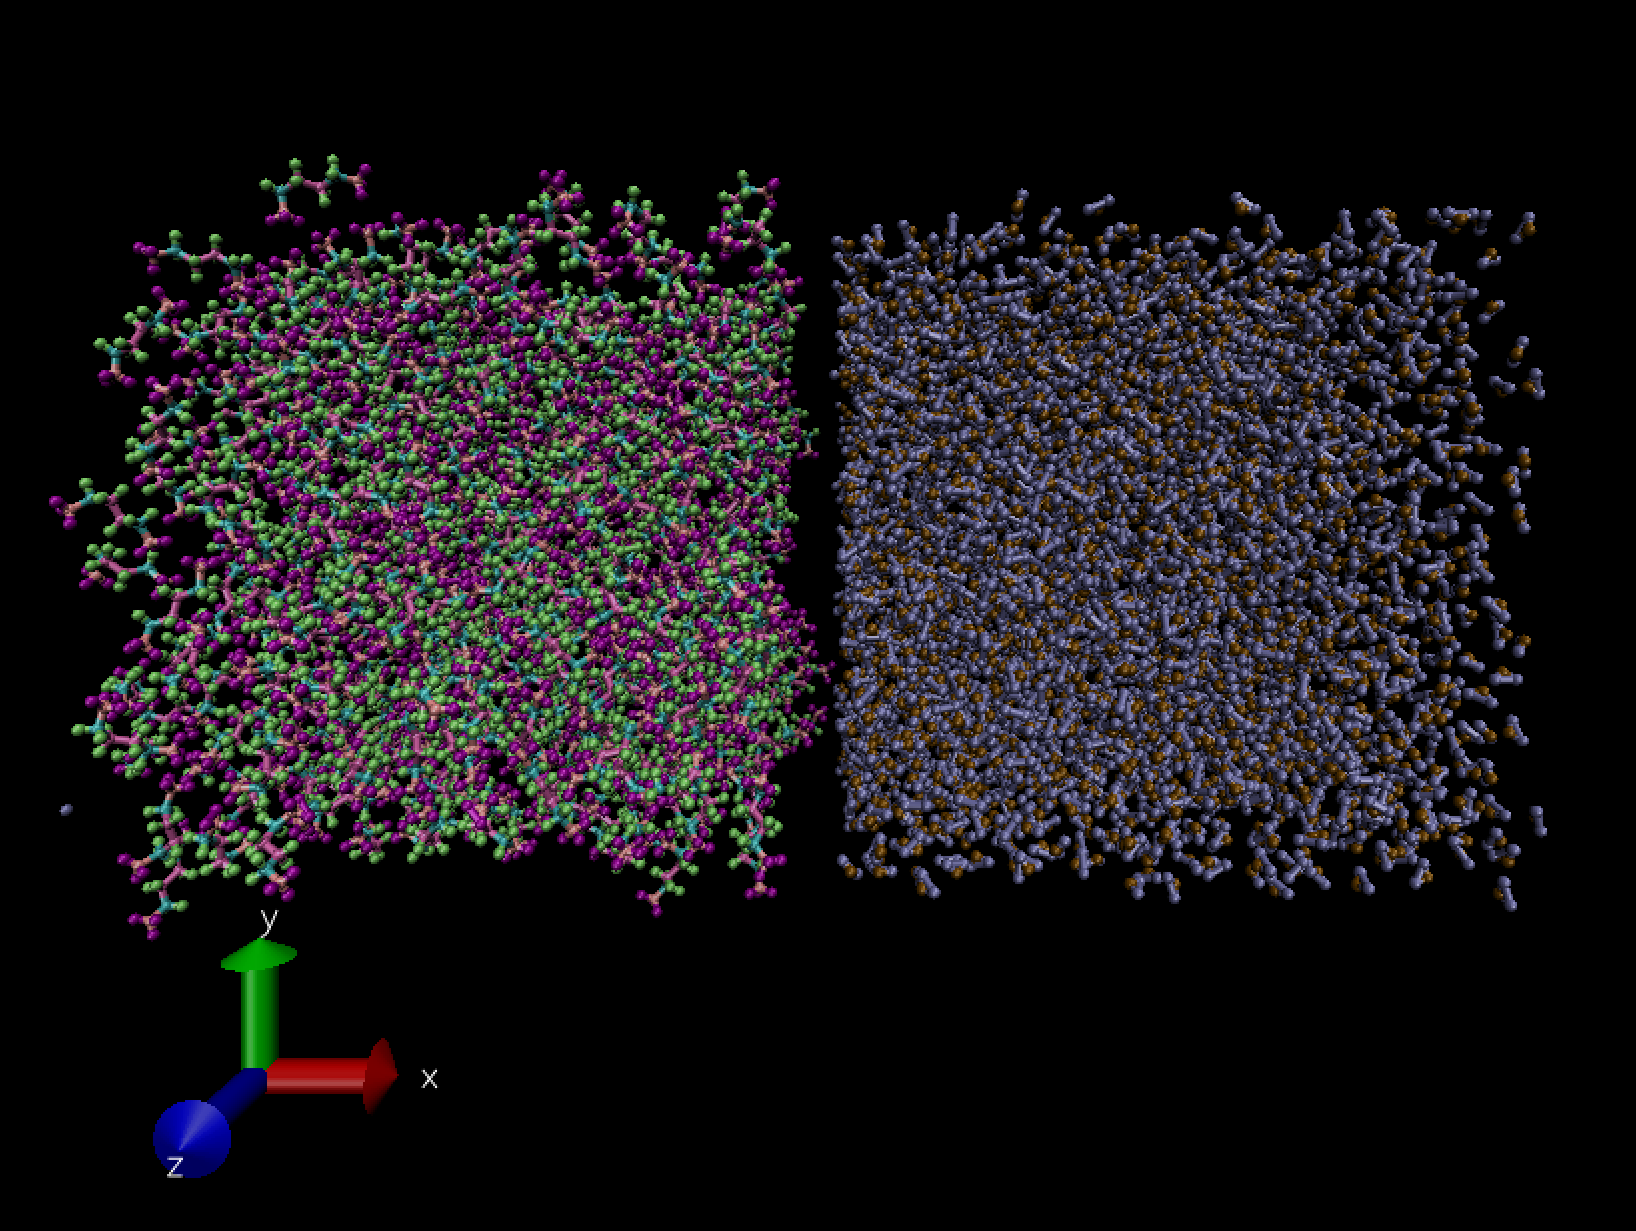
\includegraphics[scale=0.4]{lammps_taffi-tip4p2005_0}
\caption{Lammps simulation of the TAFFI - TIP4P/2005 interface.  Arithmetic mixing, 200,000 time steps.  This is the 0th timestep.}
\end{figure}

After 200,000 time steps:

\begin{figure}[H]
\centering
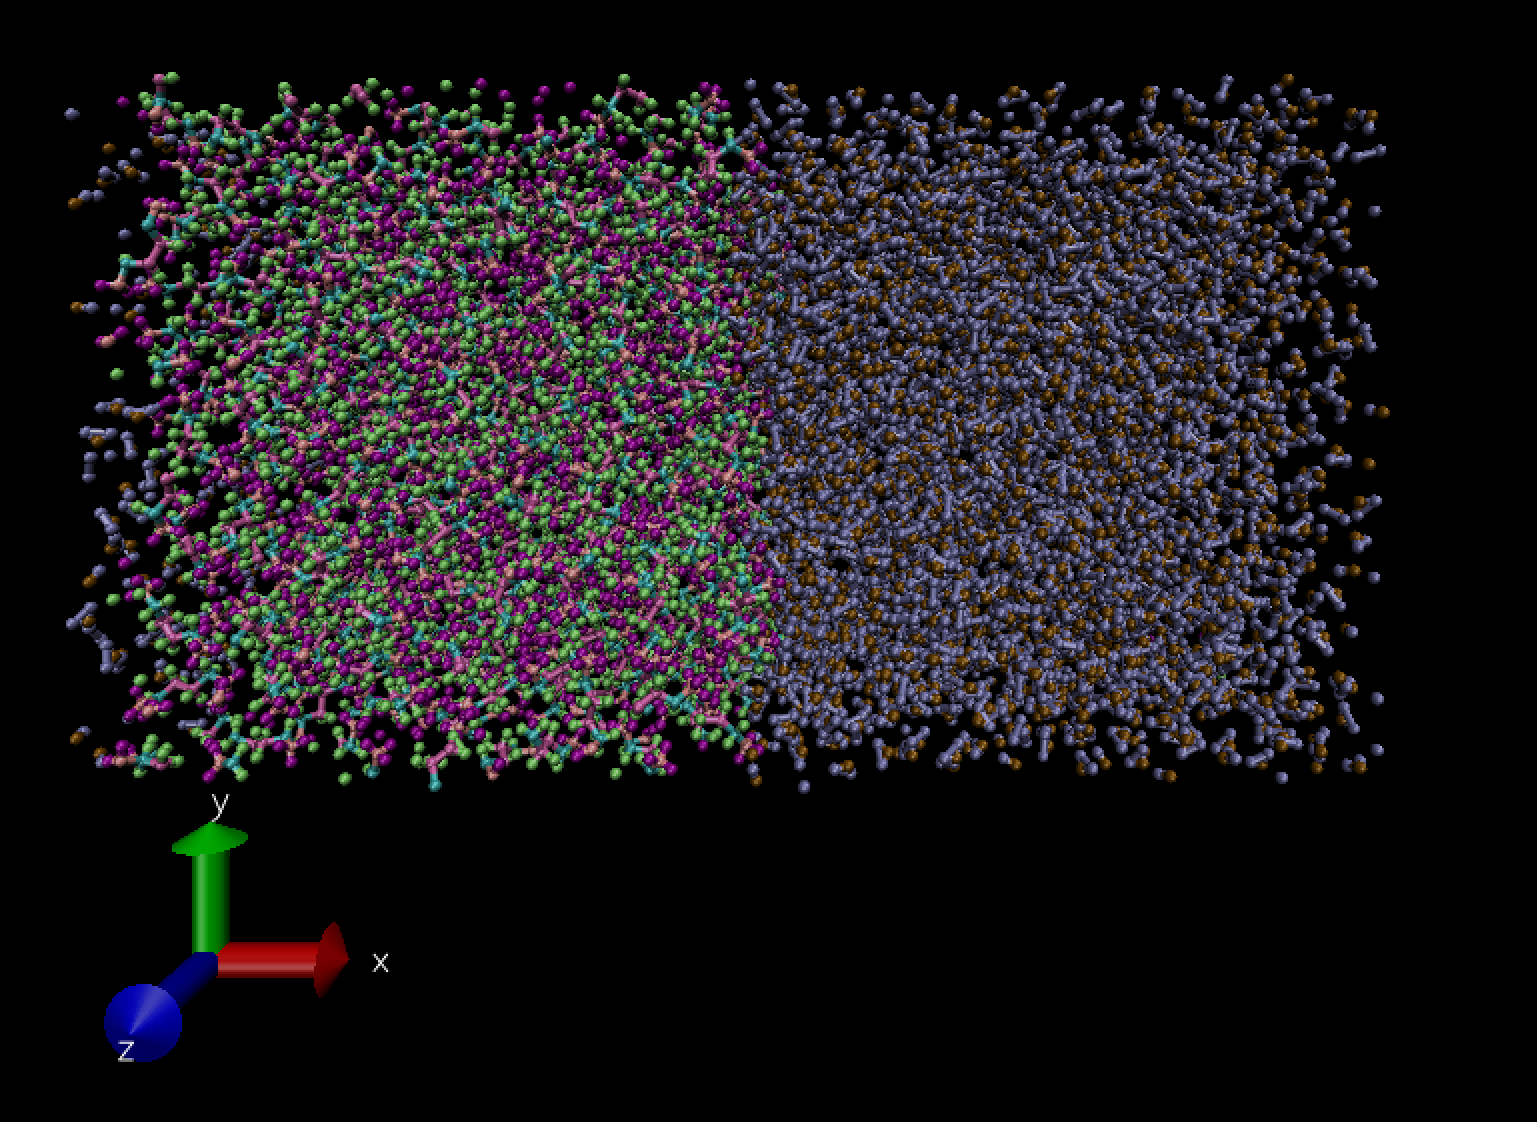
\includegraphics[scale=0.4]{lammps_taffi-tip4p2005_200000}
\caption{Lammps simulation of the TAFFI - TIP4P/2005 interface.  Arithmetic mixing, 200,000 time steps.  This is the 199,000th timestep.}
\end{figure}

For more direct comparison, here is the dash version of TAFFI + TIP4P/F at 200,000 steps:

\begin{figure}[H]
\centering
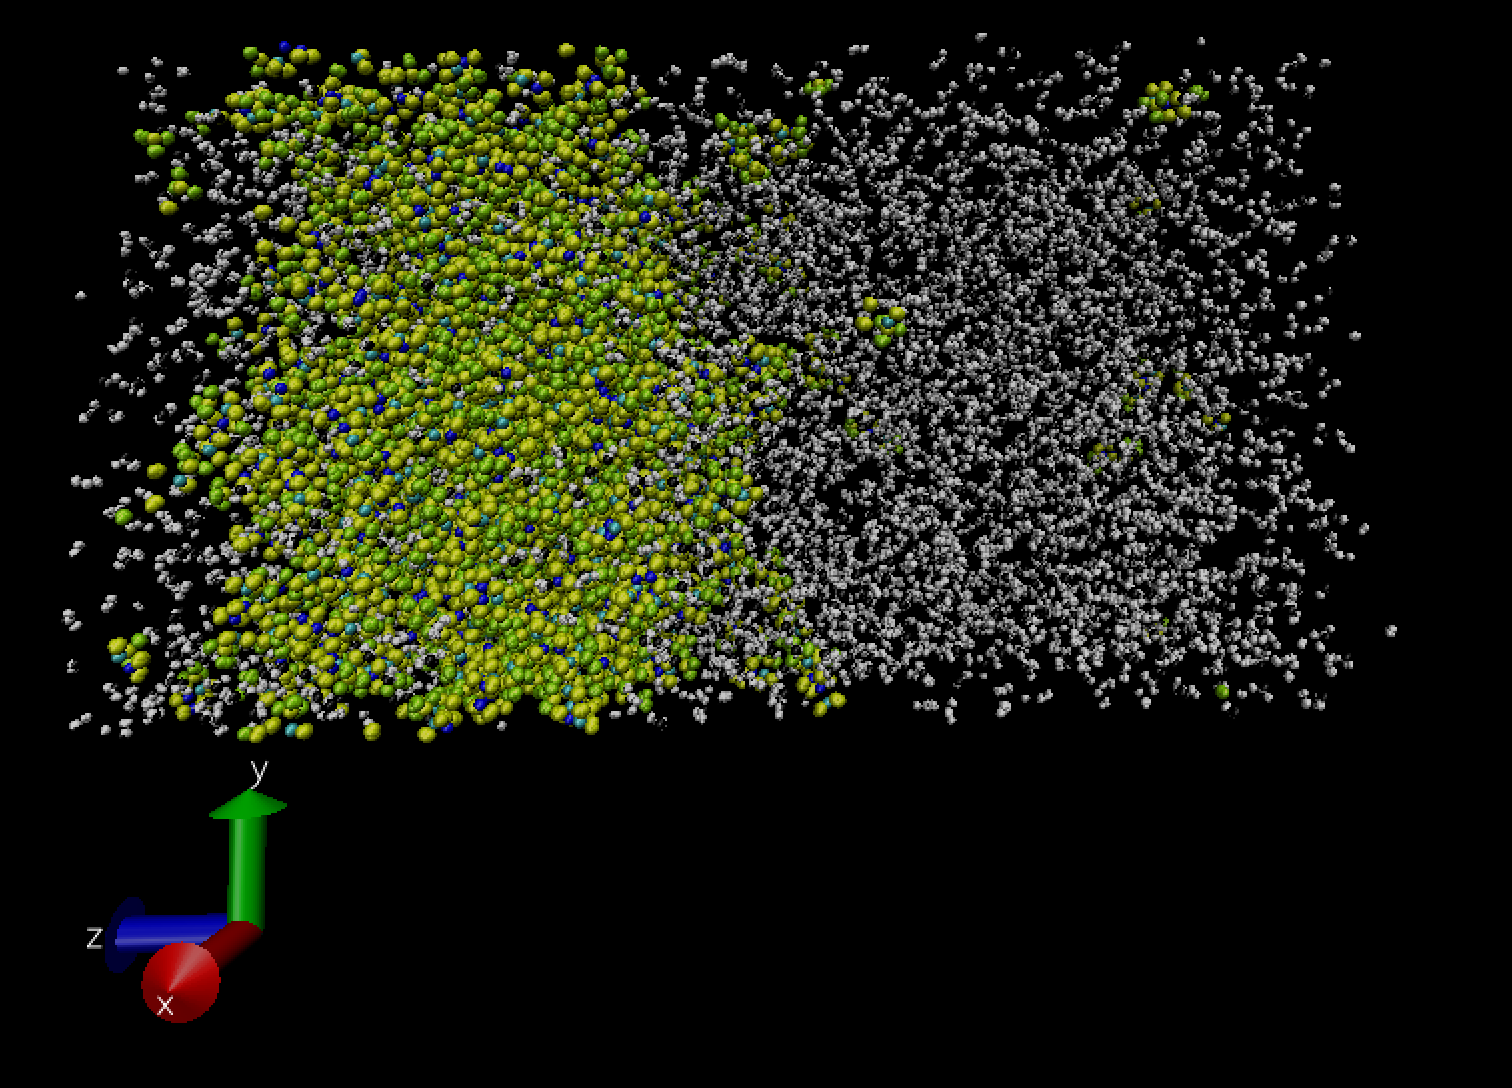
\includegraphics[scale=0.4]{dash_taffi-tip4pF_8beads_200000}
\caption{DASH simulation of the TAFFI - q-TIP4P/F interface.  Arithmetic mixing, 4,000,000 time steps.  This is the 3,950,000th timestep.}
\end{figure}

\item Now, we are going to construct the TIP4P/F in LAMMPS.  The starting point is the TIP4P/2005 classical rigid water model, which we have already implemented.  The next step is to add a quartic expansion of a Morse potential for the OH stretch:
\begin{align}
\begin{split}
V_{OH}(r) = D_r\left[\alpha_r^2(r - r_0)^2 - \alpha_r^3(r - r_0)^3 + \frac{7}{12}\alpha_r^4(r - r_0)^4\right], 
\end{split}
\end{align}
where $D_r = 116.09$, $\alpha_r = 2.287$, and $r_0 = 0.9419$.  

And then we add a simple harmonic potential for the bond angle:

\begin{align}
\begin{split}
V_{HOH}(\theta) = \frac{1}{2}k_\theta(\theta - \theta_0)^2, 
\end{split}
\end{align}
where $k_\theta = 87.85$, and $\theta_0 = 107.4$.


\item In LAMMPS, then, we will try using bond\_style class2 for the quartic expansion of the Morse potential for the OH stretch:

\begin{align}
\begin{split}
E = K_2(r - r_0)^2 + K_3(r - r_0)^3 + K_4(r - r_0)^4,
\end{split}
\end{align}
where $r_0 = r_{eq}$, $K_2 = \alpha_r^2 = 5.23$, $K_3 = -\alpha_r^3 = -11.962$, and $K_4 = \frac{7}{12}\alpha_r^4 = 15.958$.

\item We will use angle\_style harmonic for the simple harmonic potential for the bond angle:

\begin{align}
\begin{split}
E = K(\theta - \theta_0)^2,
\end{split}
\end{align}
where $K = \frac{1}{2}k_\theta$ and $\theta_0 = \theta_{eq} = 107.4$.  

\item Then, we created a data\_water\_flexible.txt file, which is a data file describing a single TIP4P/F water molecule for lammps.  I then created an in.water\_flexible file, a lammps input file to run the flexible water model simulation.  I modified this from the TIP4P/2005 input file by removing the fix shake command and adding the bond\_style class2 command.  I then ran lammps\_molecule\_replicator\_water.py in order to get 3650 flexible water molecules on an initial lattice.  
\item I tried running a lammps simulation using in.water\_flexible, but I am getting the error that the program does not recognize class2.  Turns out that this belongs to the LAMMPS package CLASS2, which might not be compiled for in my folder.  So checking that now.  

\item Compiled LAMMPS with CLASS2, and now able to run the flexible water model.  However, massive forces seem to be appearing as I am getting the error: "Out of range atoms - cannot compute PPPM).  It works better if I make the timestep miniscule, but it still breaks eventually.  Sometimes says missing bonds or atoms.  My guess is that I shouldn't be using the command pair\_style lj/cut/tip4p/long.  So perhaps for next time, what I need to do is just implement the water model irrespective of that particular pair style command, and instead I need to input all of the specifications by hand.  

\item Setting that aside for now, let's turn to DASH again, and try different parameter sets here.  Let's first work just in the classical world, with one bead.  First, let's run TAFFI + TIP4P/F in DASH using TAFFI parameters, geometric mixing, and 1 bead.   
\item This is currently running.
\item Now, let's run TAFFI + TIP4P/F in DASH using TAFFI parameters, arithmetic mixing, and 1 bead.  Just to check/be consistent.  
\item This is also currently running.  

 

\end{enumerate}

\subsection{2/23/2018}
\begin{enumerate}
\item NOTICED AN ERROR: MISSING FACTOR OF 116 IN THE BOND POTENTIAL.  FIX THIS NEXT. 
\end{enumerate}

\subsection{2/27/2018}
\begin{enumerate}
\item Fixed this problem, added the missing factor of 166.09 in the bond potential where it was due.  Saved the resulting new input file.  Currently, running an NPT system of 3650 water molecules in order to generate an initial configuration for the test interface of q-TIP4P/F and TAFFI in LAMMPS.  
\item The TAFFI + TIP4P/F in DASH using TAFFI parameters, arithmetic mixing, and 1 bead finished running.  There is too much mixing going on.  Here is a snapshot at time zero:

\begin{figure}[H]
\centering
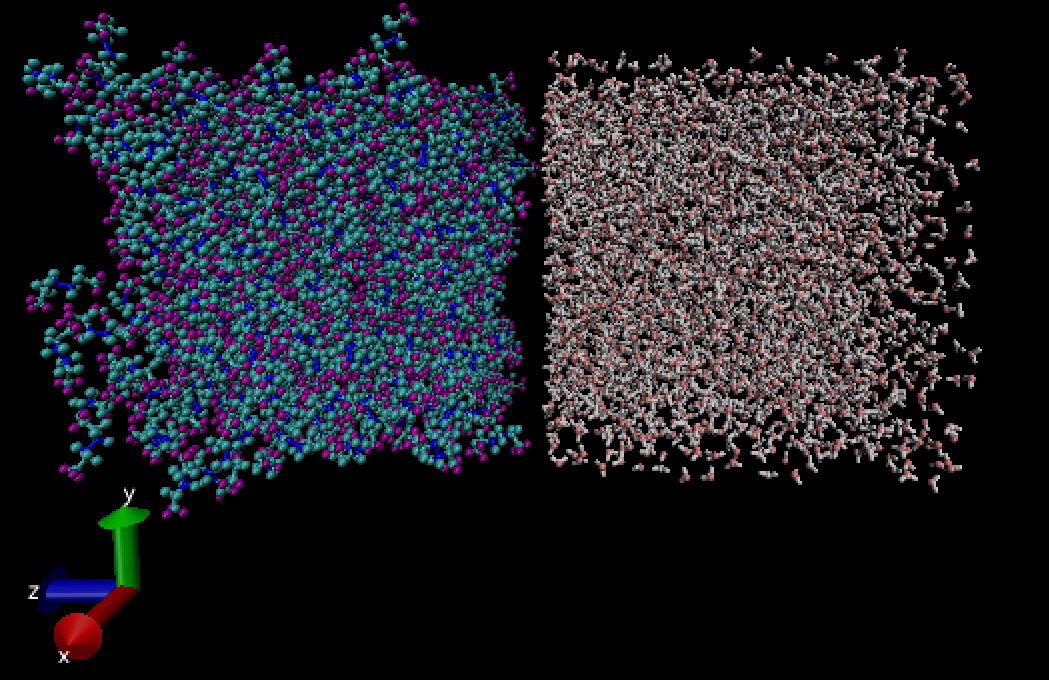
\includegraphics[scale=0.7]{dash_taffi-tip4pF_arithmetic_1bead_0}
\caption{DASH simulation of the TAFFI - q-TIP4P/F interface.  Arithmetic mixing, 4,000,000 time steps, 1 bead.  This is the 0th timestep.}
\end{figure}

\item Here is a snapshot after 4,000,000 timesteps of length 0.5:
\begin{figure}[H]
\centering
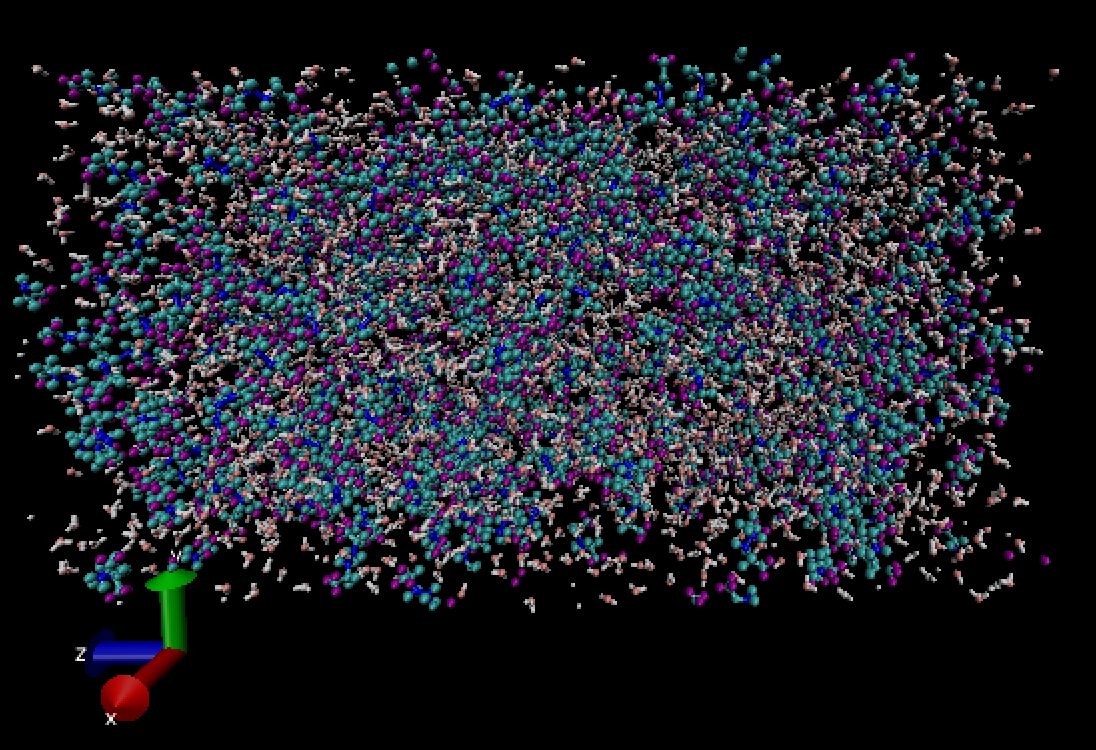
\includegraphics[scale=0.7]{dash_taffi-tip4pF_arithmetic_1bead_3950000}
\caption{DASH simulation of the TAFFI - q-TIP4P/F interface.  Arithmetic mixing, 4,000,000 time steps, 1 bead.  This is the 3950000th timestep.}
\end{figure}

\item The TAFFI + TIP4P/F in DASH using TAFFI parameters, geometric mixing, and 1 bead also finished running.  There is too much mixing.  Here is a snapshot at time zero:

\begin{figure}[H]
\centering
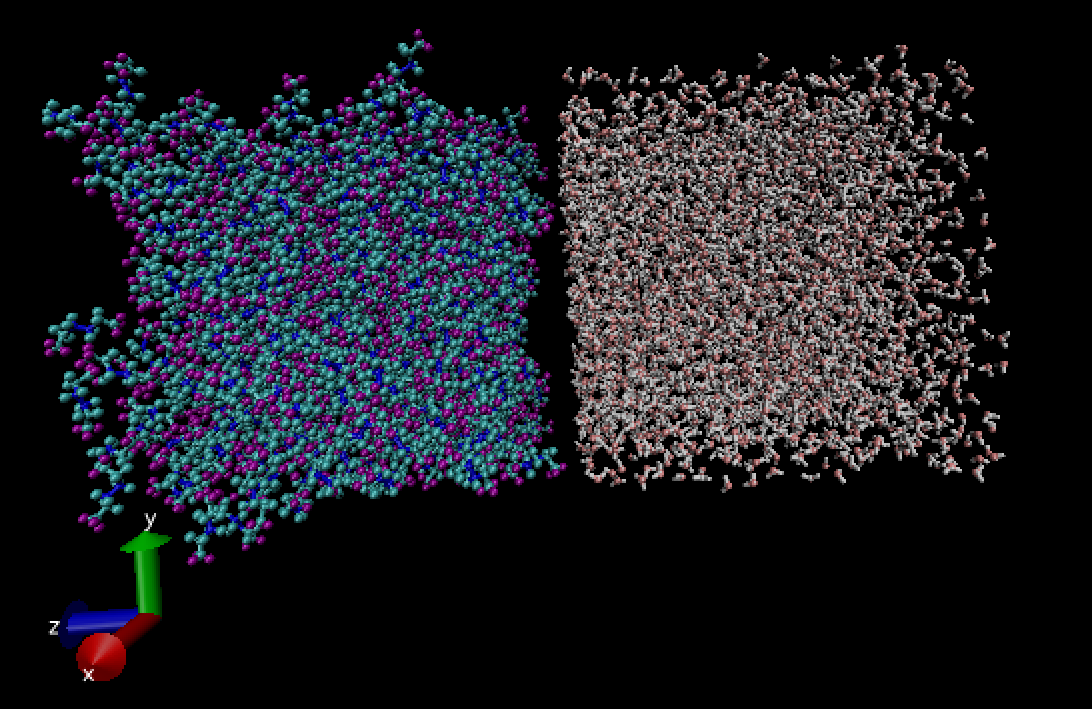
\includegraphics[scale=0.7]{dash_taffi-tip4pF_geometric_1bead_0}
\caption{DASH simulation of the TAFFI - q-TIP4P/F interface.  Geometric mixing, 4,000,000 time steps, 1 bead.  This is the 0th timestep.}
\end{figure}

\item Here is after 4,000,000 timesteps of length 0.5:

\begin{figure}[H]
\centering
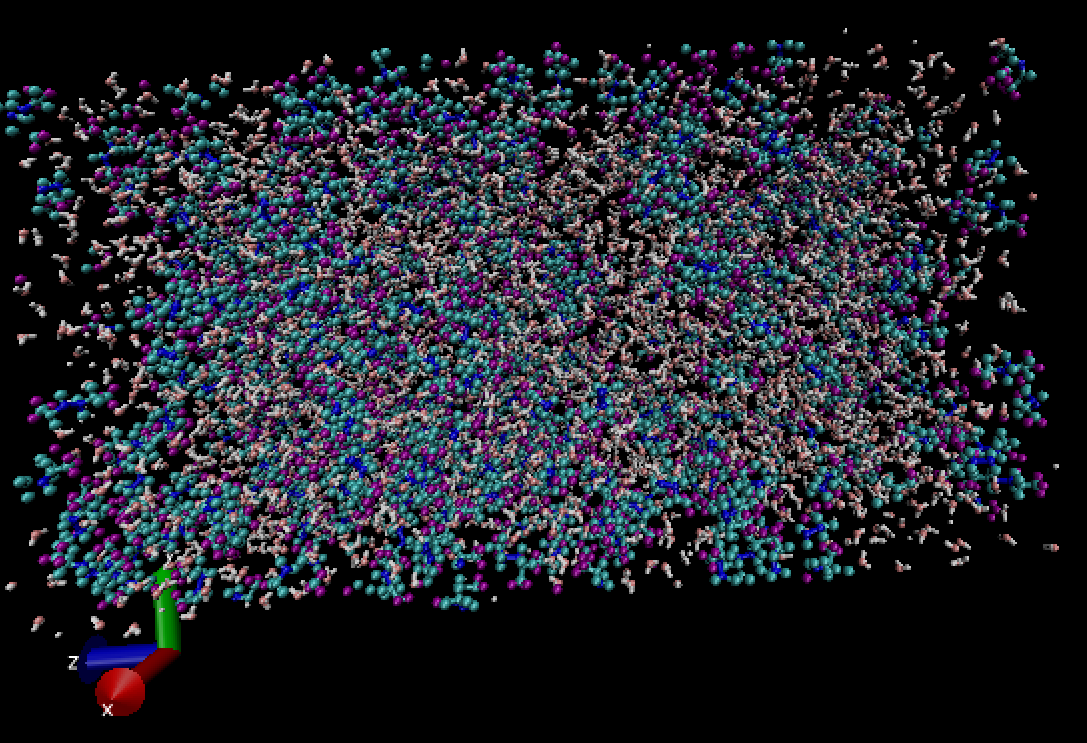
\includegraphics[scale=0.7]{dash_taffi-tip4pF_geometric_1bead_3950000}
\caption{DASH simulation of the TAFFI - q-TIP4P/F interface.  Geometric mixing, 4,000,000 time steps, 1 bead.  This is the 3950000th timestep.}
\end{figure}
  
\end{enumerate}



\subsection{3/5/2018}
\begin{enumerate}
\item Downloaded the trajectory file, dump.water\_flexible.lammpstrj, from the lammps\_work/water folder to check the performance of the TIP4P/F in LAMMPS.  The trajectory looks good.  Moreover, the density of th system reached a final value instantaneous value, at step 200,000, of 0.98752919.  The output file produced, output\_water\_flexible\_preequil.txt, taken after the final 200,000th step in the simulation, also looks reasonable:

 \begin{figure}[H]
\centering
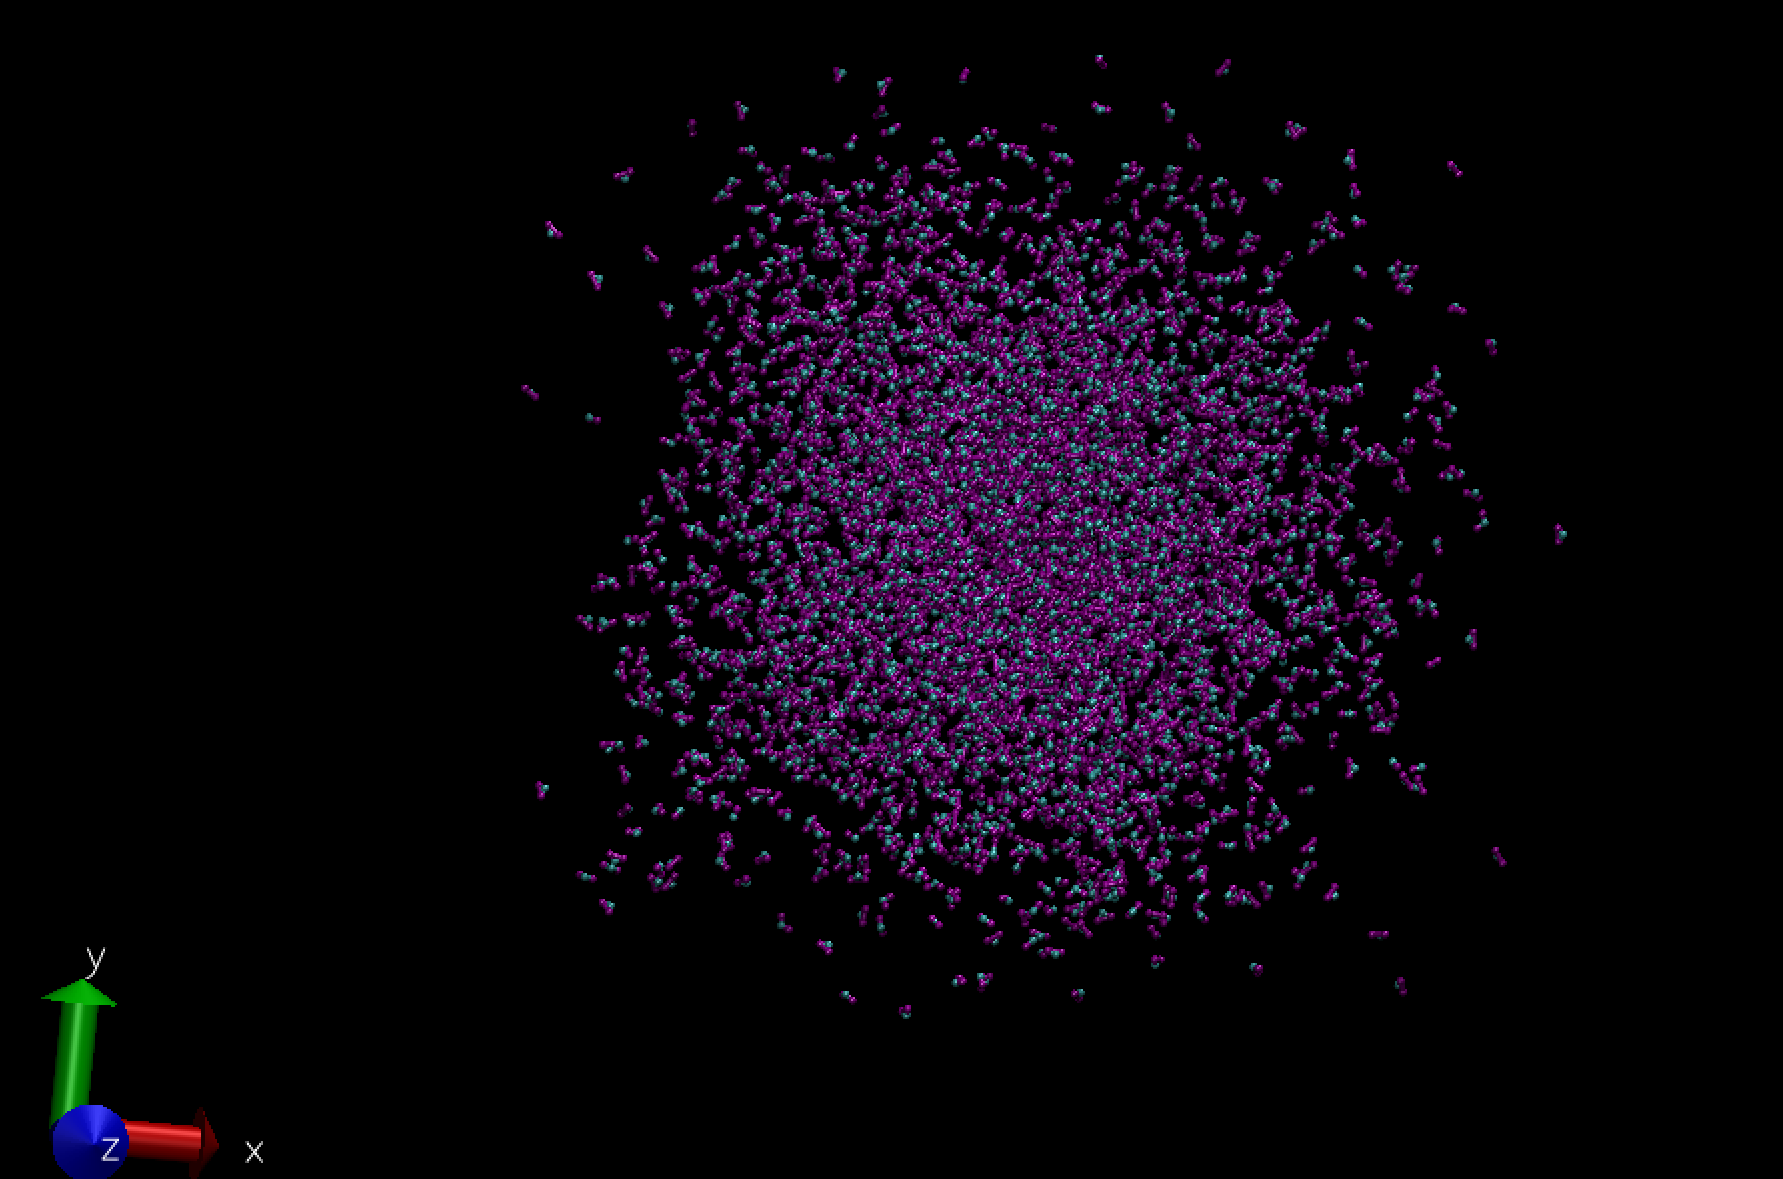
\includegraphics[scale=0.4]{lammps_tip4pF_200000}
\caption{LAMMPS simulation of TIP4P/F water.  Geometric mixing, 200,000 timesteps, this is the final step.}
\end{figure}

\item Now, we will follow steps from before to simulate the TAFFI - q-TIP4P/F interface in LAMMPS.  
\item First, move output\_water\_flexible\_preequil.txt into the interface folder.  Also move the file hexane\_restart\_modified.txt, which is  a preequilibrated slab of TAFFI hexane.  Now, we have two preequilibrated slabs - one with 500 TAFFI hexane molecules, and the other with 3650 TIP4P/F water molecules. 
\item Second, move original molecular data file descriptions of single molecules of TAFFI hexane (i.e. data\_webb\_hexane\_modified.txt) and TIP4P/F water (data\_water\_flexible.txt) to the interface folder.  
\item Run the file lammps\_molecule\_replicator\_tip4pwater\_webbhexane.py in order to produce a mixed system template that can be used as the -dataoriginal input file in the lammps\_restart.py program.  This is what this original file looks like:

\begin{figure}[H]
\centering
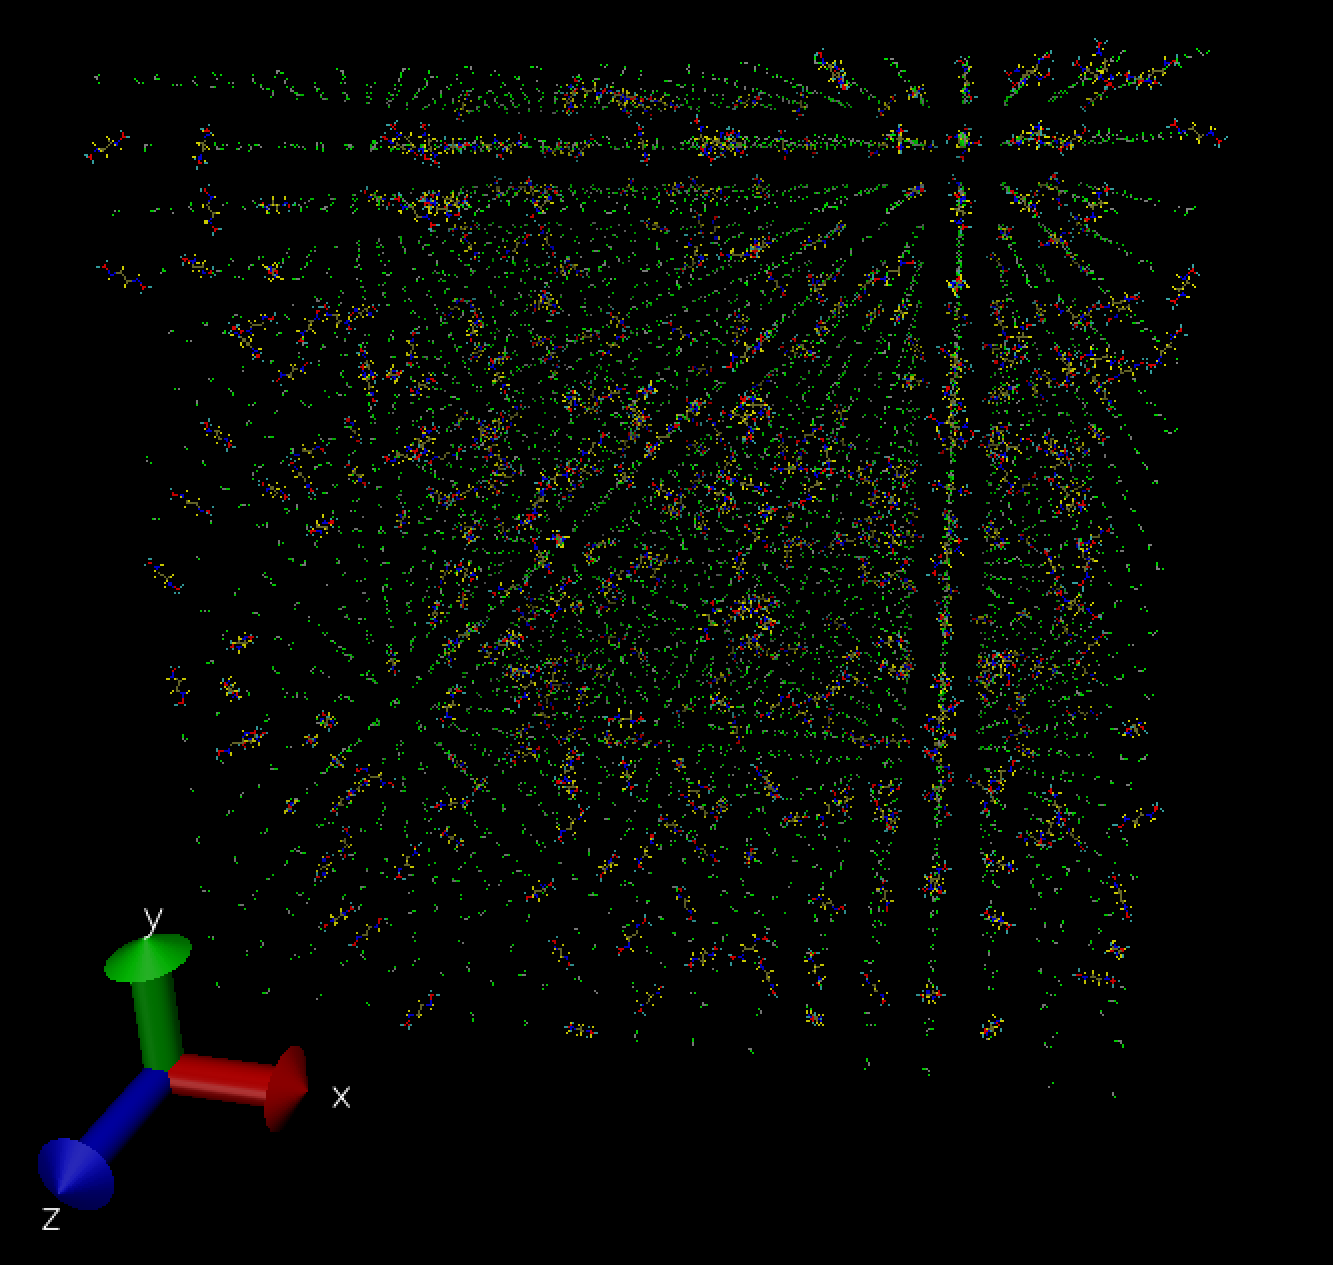
\includegraphics[scale=0.4]{datafileoriginal_taffi_tip4pF}
\caption{Image of datafileoriginal for TAFFI and TIP4P/F.}
\end{figure}

Run the lammps\_restart.py file using -data1=hexane\_restart\_modified.txt, -data2=output\_water\_flexible\_preequil.txt, and -dataoriginal=datafileoriginal\_taffi\_tip4pF.txt.  This produces the initial configuration for the hexane-water TAFFI-TIP4P/F system in LAMMPS:

\begin{figure}[H]
\centering
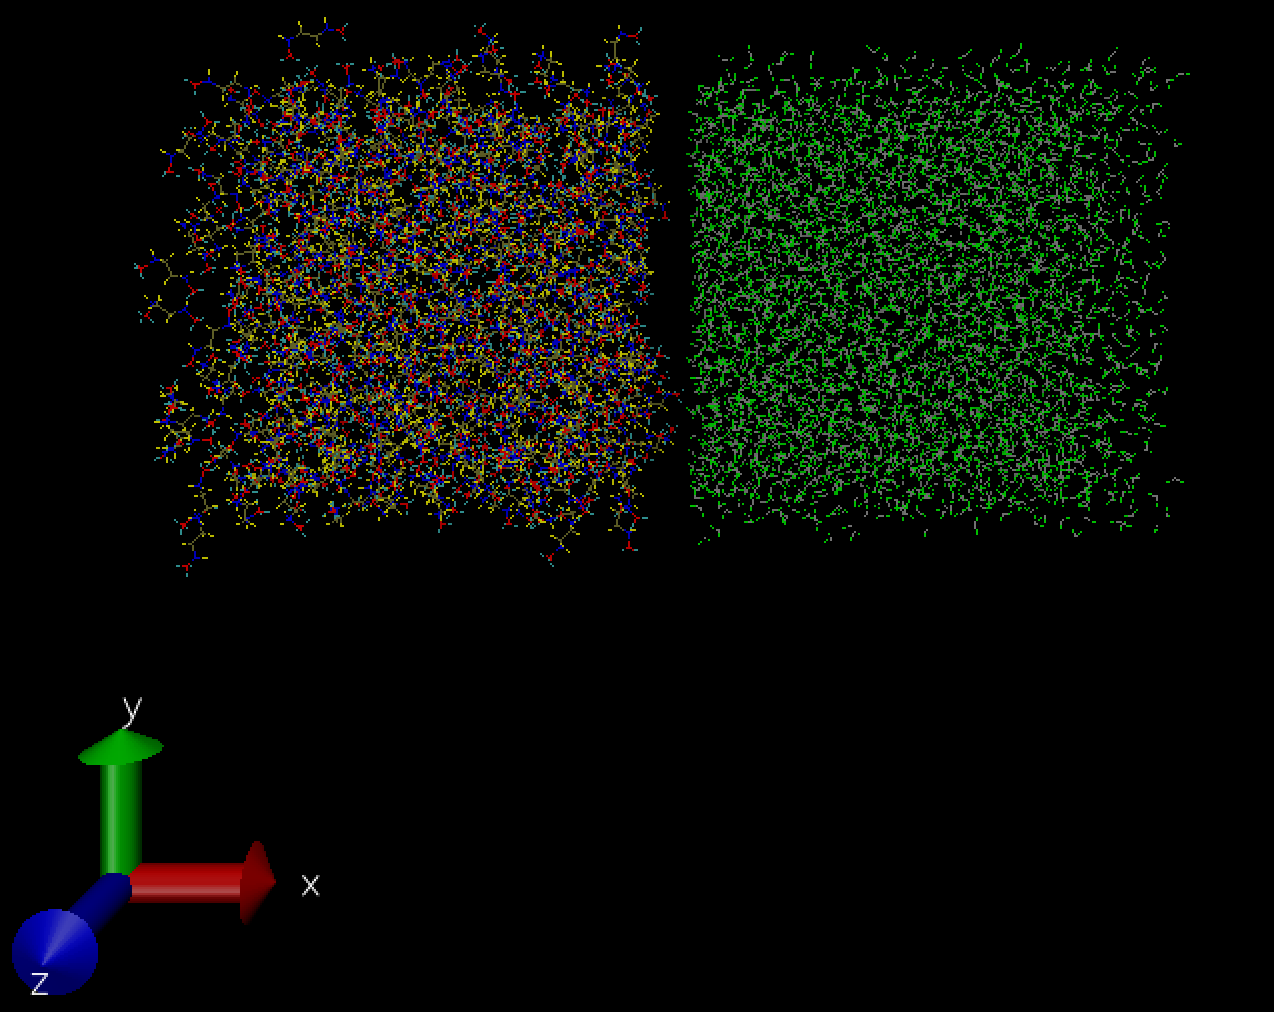
\includegraphics[scale=0.4]{input_restart_taffi_tip4pF}
\caption{Image of input file for TAFFI and TIP4P/F.}
\end{figure}

\item Finally, adjust the input\_restart\_taffi\_tip4pF file to have a Bond Coeffs style that is compatible with bond\_style class2.  

\item HYPOTHESIS: All of my previous LAMMPS	 simulations of the interface were NPT, while in DASH, they were NVT.  Perhaps this is a difference?  I must do all simulations in both to check...

\item I am now running a LAMMPS simulation of the hexane-water interface: 500 TAFFI hexane, 3650 TIP4P/F water, arithmetic mixing, NPT, 200,000 steps of time 1.0.  

\item I am now also running an NVT LAMMPS simulation of the hexane-water interface: 500 TAFFI hexane, 3650 TIP4P/F water, arithmetic mixing, NVT, 200,000 steps of time 1.0.   

\end{enumerate}

\subsection{3/6/2018}
\begin{enumerate}
\item These are snapshots of the NPT simulations:

\begin{figure}[H]
\centering
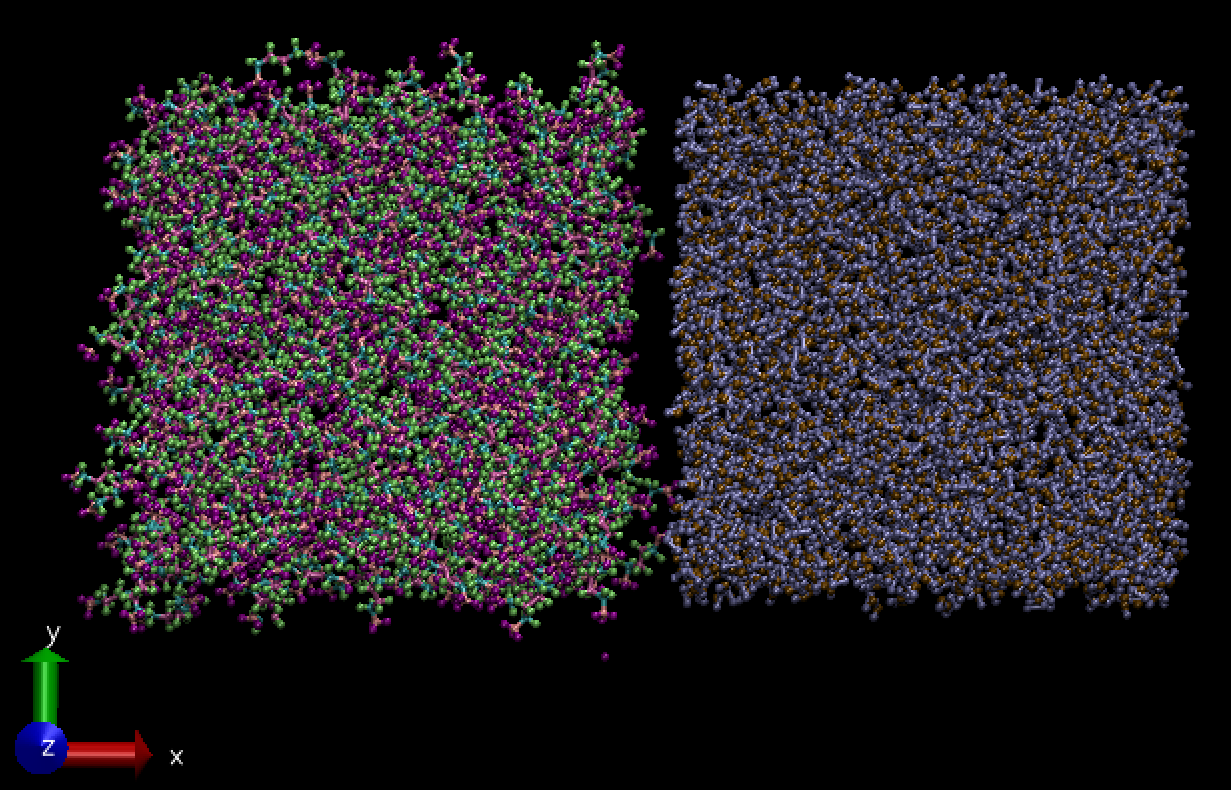
\includegraphics[scale=0.4]{lammps_taffi-tip4pF_0}
\caption{LAMMPS simmulation of 500 TAFFI hexane, 3650 TIP4P/F water, arithmetic mixing, NPT at T = 300 and P = 1, 200,000 timesteps of length 1.0 fs, NPT pre-equilibration of each slab at the same T and P.  Cutoff = 12.0, pppm/tip4p 1e-4, special bonds 0 0 0.  This is the 0th timestep.}
\end{figure}

\begin{figure}[H]
\centering
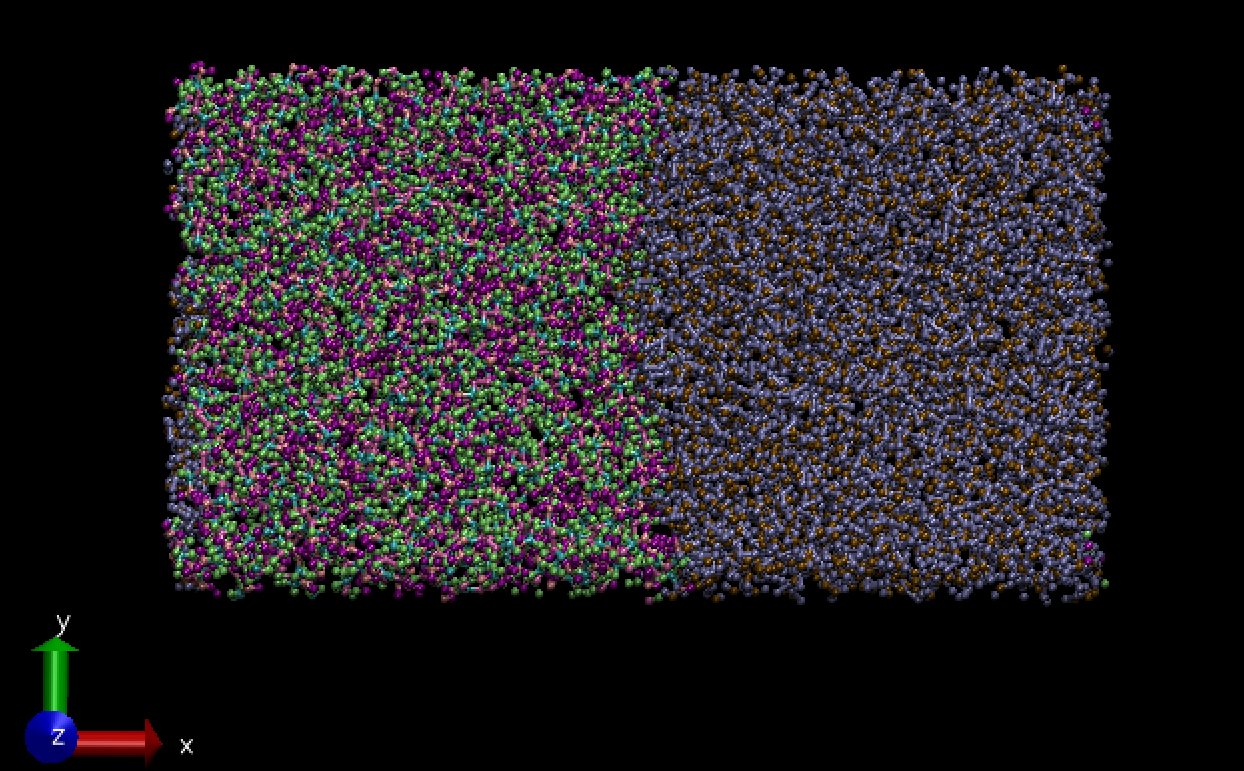
\includegraphics[scale=0.4]{lammps_taffi-tip4pF_200000}
\caption{LAMMPS simmulation of 500 TAFFI hexane, 3650 TIP4P/F water, arithmetic mixing, NPT at T = 300 and P = 1, 200,000 timesteps of length 1.0 fs, NPT pre-equilibration of each slab at the same T and P.  Cutoff = 12.0, pppm/tip4p 1e-4, special bonds 0 0 0.  This is the 200,000th timestep.}
\end{figure}

\item So, the TAFFI-TIP4P/F interface in LAMMPS appears to be stable under NPT conditions.  The final density of this simulation was around 0.854.  

\item These are snapshots of the NVT simulations: 

\begin{figure}[H]
\centering
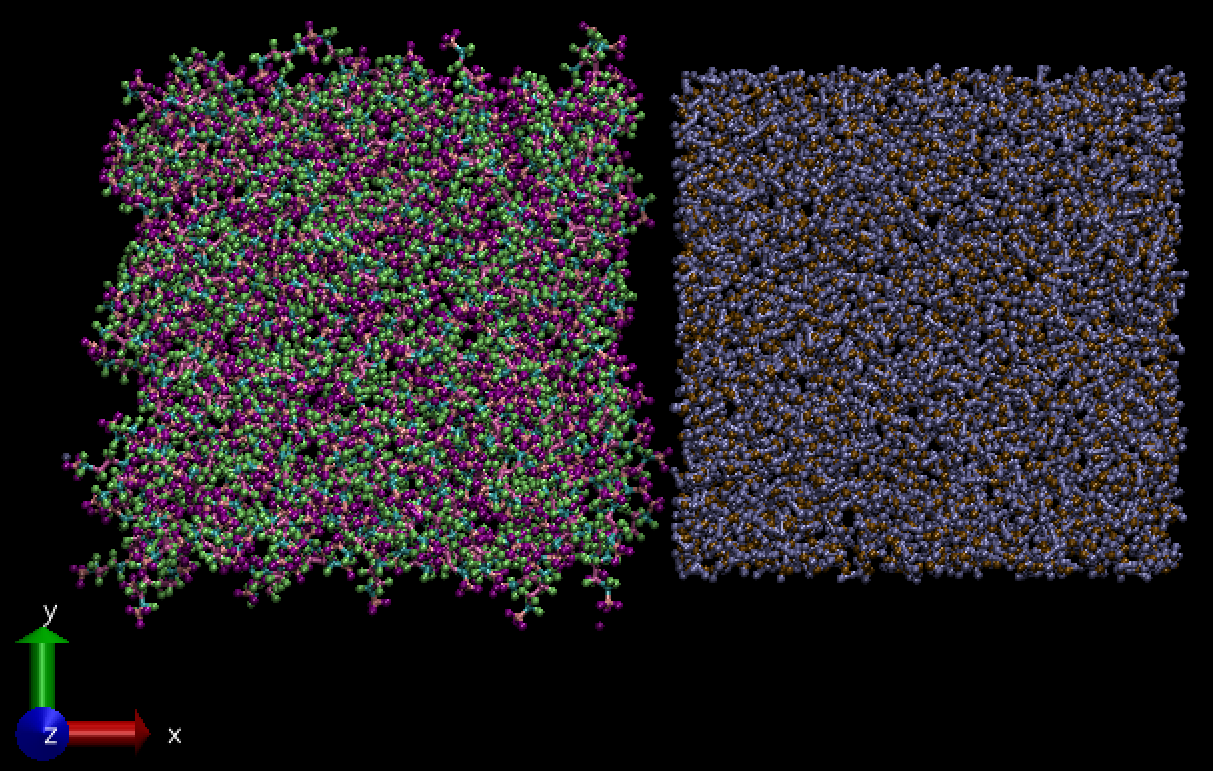
\includegraphics[scale=0.4]{lammps_taffi-tip4pF_NVT_0}
\caption{LAMMPS simmulation of 500 TAFFI hexane, 3650 TIP4P/F water, arithmetic mixing, NVT at T = 300 and V = (4.722, 5.62, 6.26) x (113.25, 64.29, 64.71), 200,000 timesteps of length 1.0 fs, NPT pre-equilibration of each slab at the same T and P = 1.0.  Cutoff = 12.0, pppm/tip4p 1e-4, special bonds 0 0 0.  This is the 0th timestep.}
\end{figure}

\begin{figure}[H]
\centering
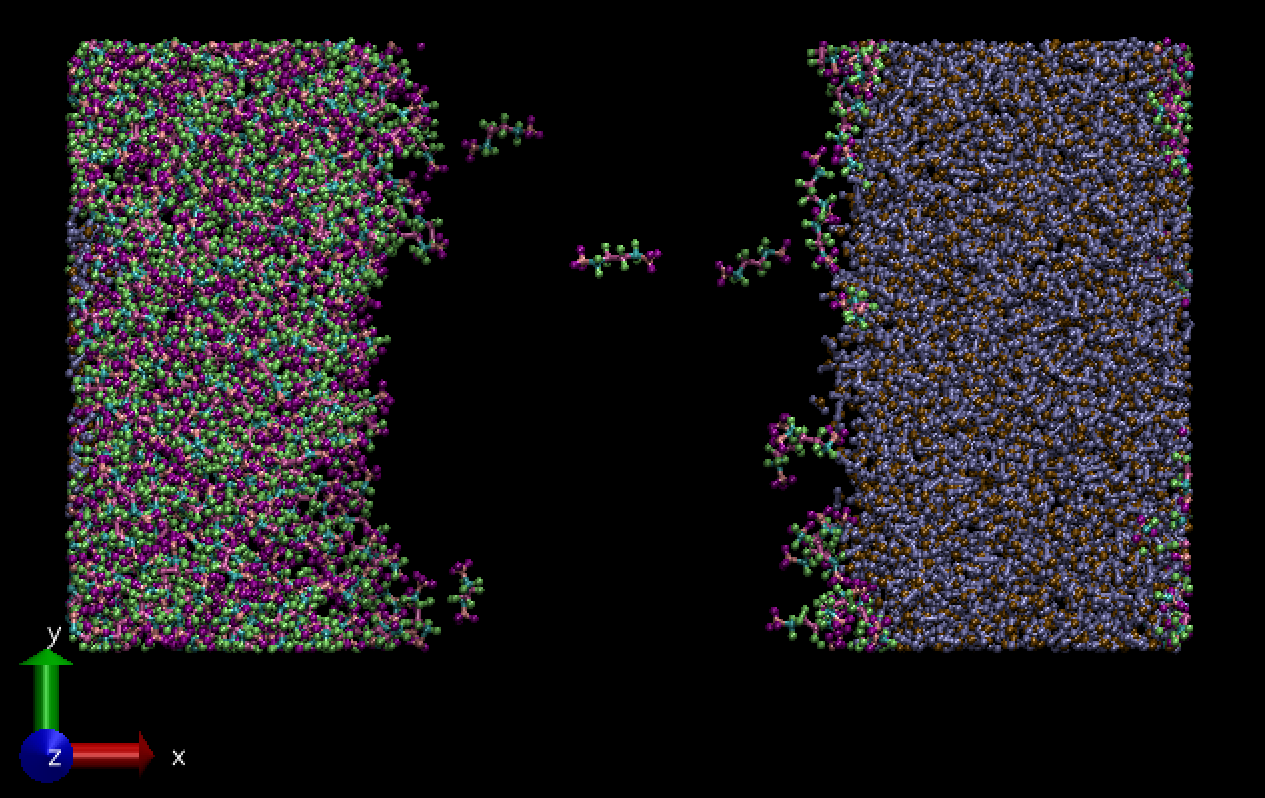
\includegraphics[scale=0.4]{lammps_taffi-tip4pF_NVT_200000}
\caption{LAMMPS simmulation of 500 TAFFI hexane, 3650 TIP4P/F water, arithmetic mixing, NVT at T = 300 and V = (4.722, 5.62, 6.26) x (113.25, 64.29, 64.71), 200,000 timesteps of length 1.0 fs, NPT pre-equilibration of each slab at the same T and P = 1.0.  Cutoff = 12.0, pppm/tip4p 1e-4, special bonds 0 0 0.  This is the 200,000th timestep.}
\end{figure}

\item I have chosen, as usual, the box bounds to be the outermost atoms.  It appears as though this results in a box that is too large for NVT to produce an actual interface in the middle.  However, an interface does exist at the x-boundaries, which appears to be stable.  The final NVT density of the simulation was around 0.4855.    

\item In order to check my new hypothesis, I want to run a classical simulation in DASH of the TAFFI-TIP4P/F interface under NPT conditions.  

These are snapshots of the NPT result:

\begin{figure}[H]
\centering
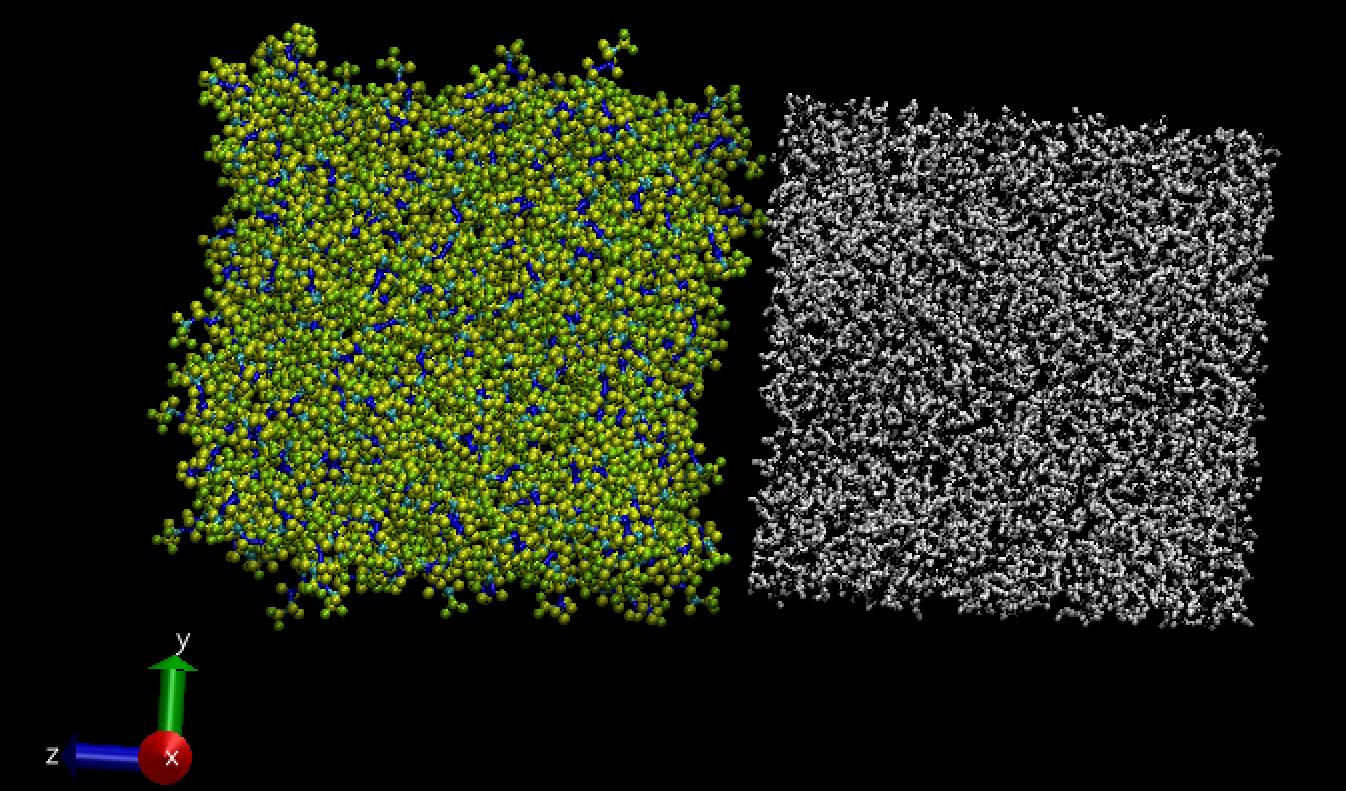
\includegraphics[scale=0.4]{dash_taffi-tip4pF_classical_NPT_0}
\caption{DASH simmulation of 500 TAFFI hexane, 3650 TIP4P/F water, arithmetic mixing, NPT Andersen/Berendsen at T = 300 and P = 1, 200,000 timesteps of length 1.0 fs, NPT pre-equilibration of each slab at 298.15K and same P.  Cutoff = 12.0, Ewald summation.  This is the 0th timestep.}
\end{figure}

\begin{figure}[H]
\centering
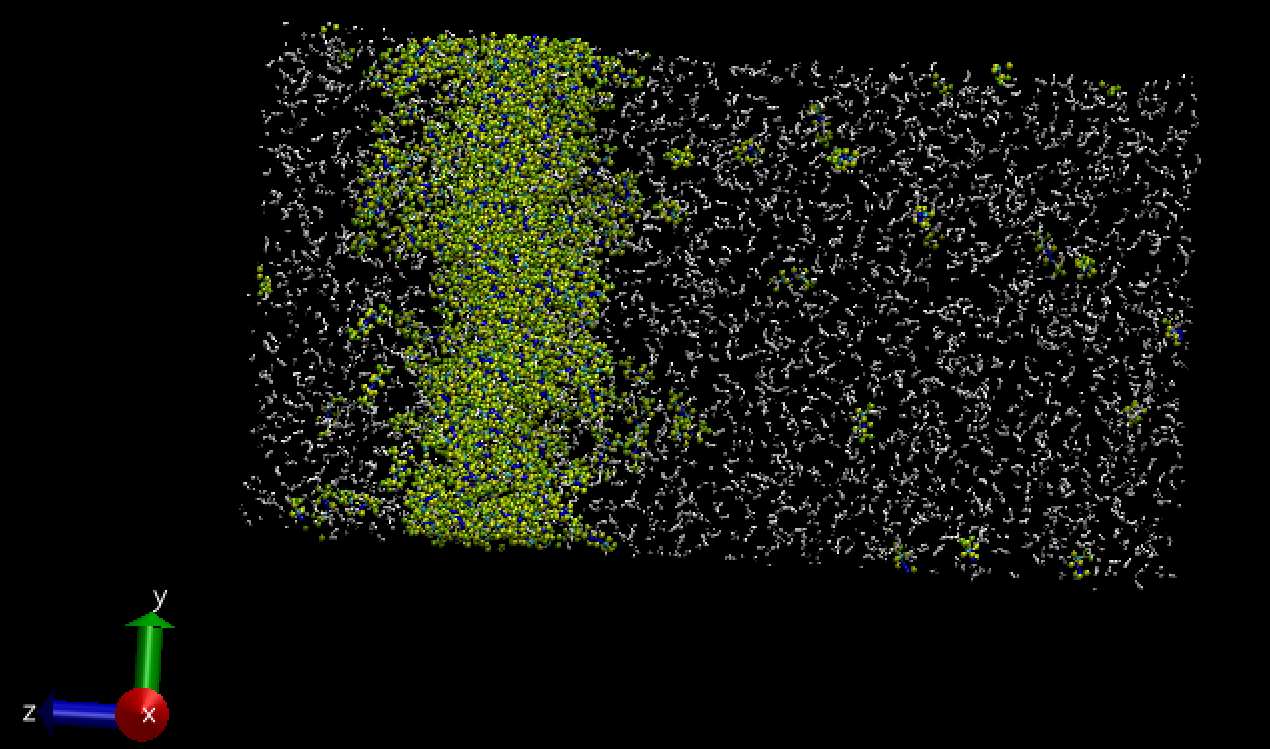
\includegraphics[scale=0.4]{dash_taffi-tip4pF_classical_NPT_200000}
\caption{DASH simmulation of 500 TAFFI hexane, 3650 TIP4P/F water, arithmetic mixing, NPT Andersen/Berendsen at T = 300 and P = 1, 200,000 timesteps of length 1.0 fs, NPT pre-equilibration of each slab at 298.15K and same P.  Cutoff = 12.0, Ewald summation.  This is the 200000th timestep.}
\end{figure}

\item There is a significant difference in the LAMMPS and DASH simulations, suggesting that something is amiss in the DASH program.  

\item I will now check over the interface\_NPT.py script to see if there are any possible sources of error.  We should check: relationship of bulk hexane and water to temperature in DASH, and compared to LAMMPS, as well as specifications of both models, i.e. charge and other parameters.  

\item Went through the interface\_NPT.py file in detail.  Did not find any errors.

\item Now, I am going to run the interface\_NPT.py file with pure water, removing the hexane component, and check the resulting density at various temperatures.  I will then do the same with hexane, removing the water.  Unless I've found the error at this point, I will then do the same calculations in LAMMPS and compare.  

\item It looks like there is an issue with the water.  So, we will start tomorrow with an exploration of what is going on with the pure water restart.  The goal will be to create a water restart within the interface framework that does not have any issues.  

\end{enumerate}

\subsection{3/7/2018}
\begin{enumerate}
\item Looking into pure water simulations in DASH.  
\item First, starting in dash\_work/water folder, running a test version of in.tip4pF.py.  
\item Ran the simulation for 100,000 steps using time length 0.5.  Density approached values aroun 0.98/0.99 by at least before 50,000 steps.  Simulation video looked reasonable.    
\item Ran a restart simulation for 50,000 steps, starting at the previous simulation's 50,000th step.  Density approached 0.985 after the 50,000 steps, which is good.  Video also looks very reasonable.  
\item Tomorrow, I will start with the file in.tip4pF\_restart7.5.py and build from it the hexane-water simulation, checking videos/densities at each step to see where things go wrong!  
\end{enumerate}

\subsection{3/15/2018}
\begin{enumerate}
\item Solved the problem.  The Ewald summation fix was not being activated.  ALL fixes must be activated in DASH.
\item To confirm, currently running: DASH simulation of 500 TAFFI hexane, 4650 TIP4P/F water, arithmetic mixing, NPT Andersen/Berendsen at T = 298.15 K and P = 1.0, 400,000 simulation steps of length 0.5 fs, NPT pre-equilibration of each slab at 298.15 K and 1.0 atm.  Potential cutoff at 12.0, long-range Ewald summation.  Classical simulation, no path integrals.     
\end{enumerate}

\subsection{3/22/2018}
\begin{enumerate}
\item Simulation above finished.  Results are shown below.  The simulation looks clean: 

\begin{figure}[H]
\centering
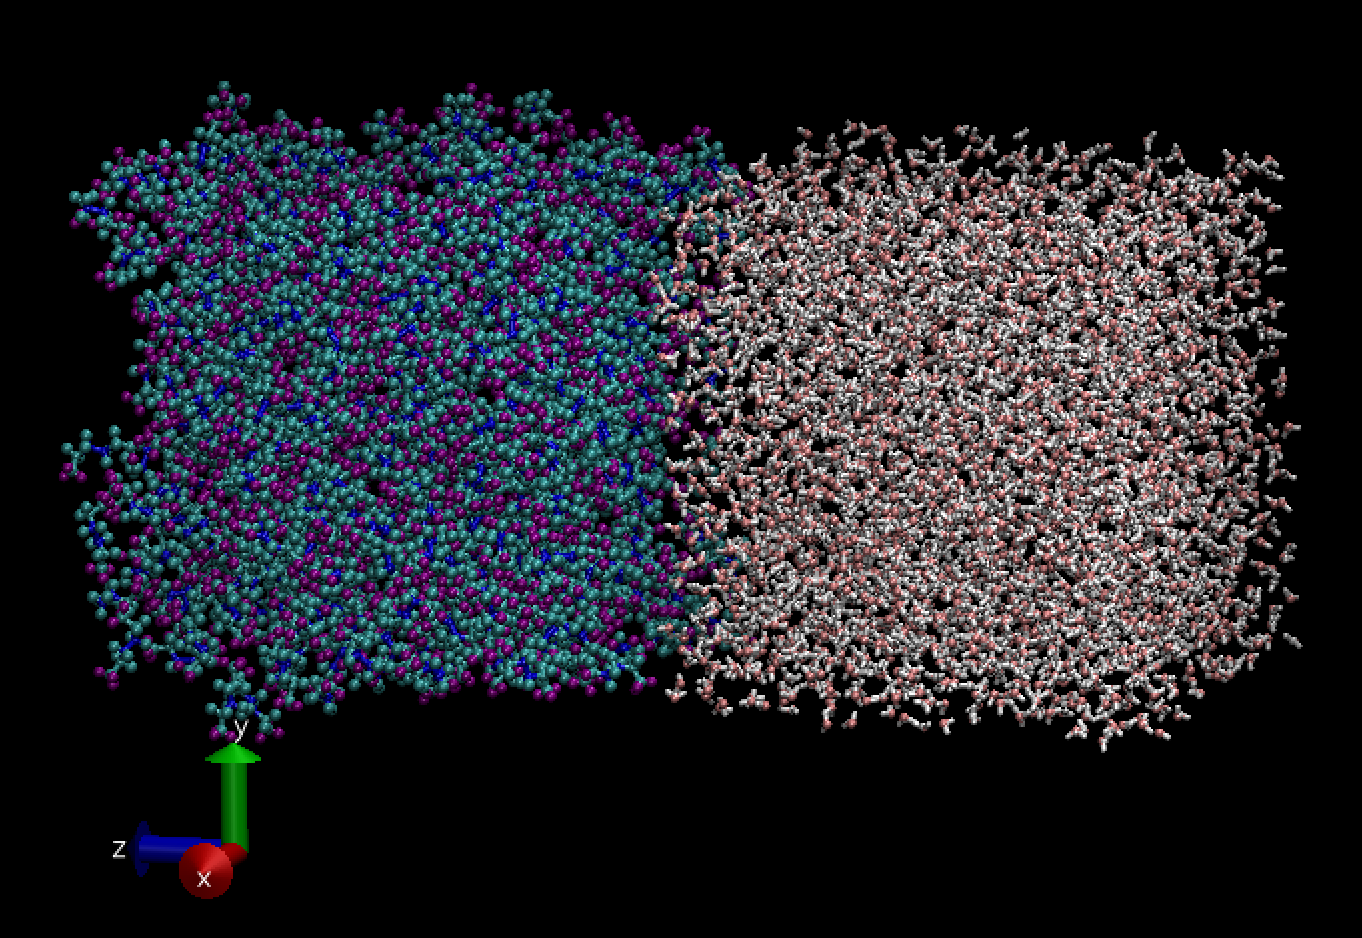
\includegraphics[scale=0.4]{dash_taffi-tip4pF_classical_arithmetic_NPT_0}
\caption{DASH simmulation of 500 TAFFI hexane, 3650 TIP4P/F water, arithmetic mixing, NPT Andersen/Berendsen at T = 298.15K and P = 1 atm, 240,000 timesteps of length 0.5 fs, NPT pre-equilibration of each slab at 298.15K and same P.  Cutoff = 12.0, Ewald summation.  Classical simulation, no path integrals.  This is the 0th timestep.}
\end{figure}

\begin{figure}[H]
\centering
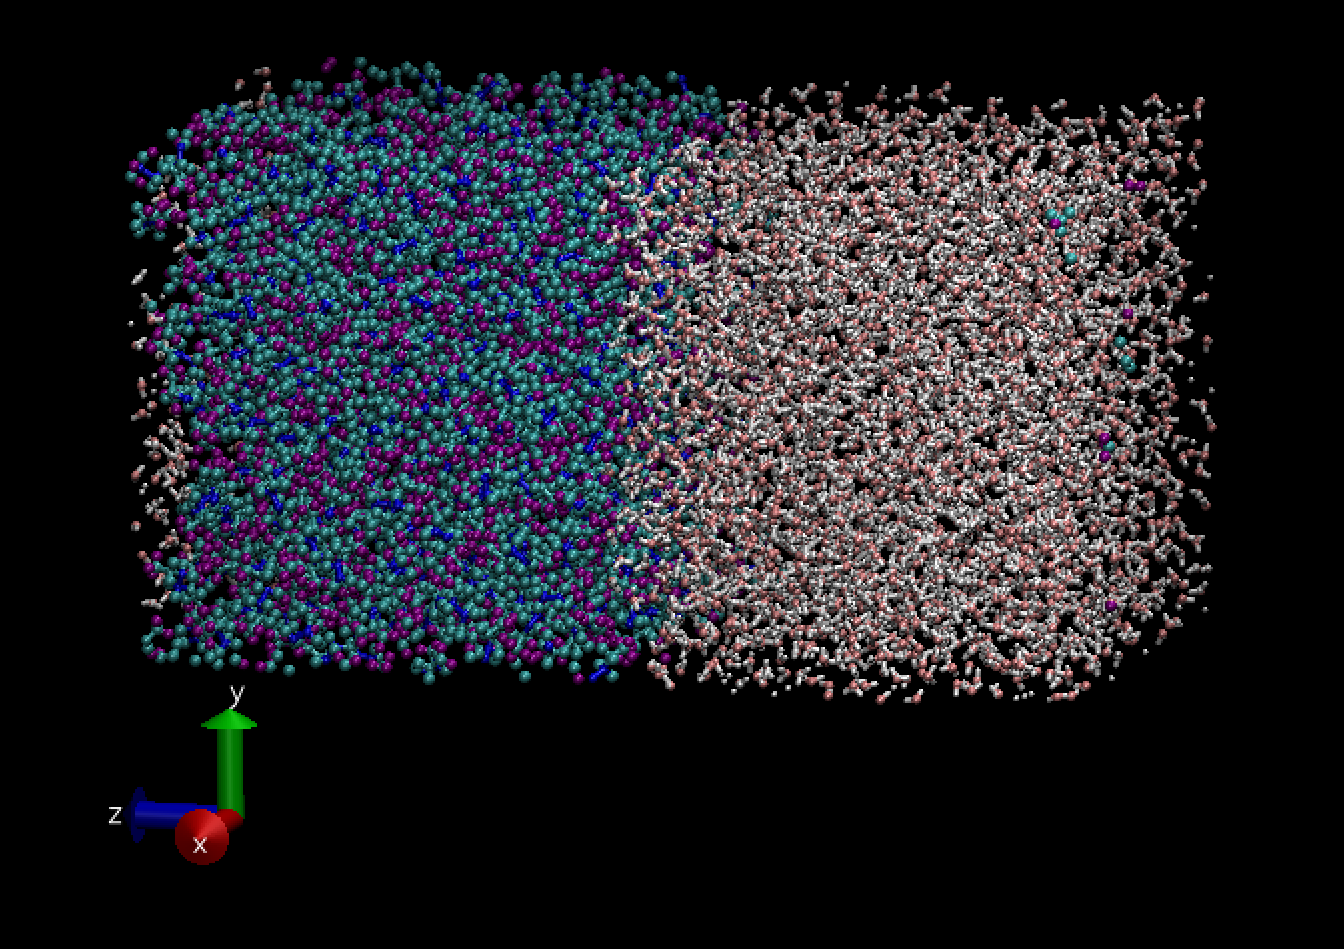
\includegraphics[scale=0.4]{dash_taffi-tip4pF_classical_arithmetic_NPT_400000}
\caption{DASH simmulation of 500 TAFFI hexane, 3650 TIP4P/F water, arithmetic mixing, NPT Andersen/Berendsen at T = 298.15K and P = 1 atm, 240,000 timesteps of length 0.5 fs, NPT pre-equilibration of each slab at 298.15K and same P.  Cutoff = 12.0, Ewald summation.  Classical simulation, no path integrals.  This is the 400,000th timestep.}
\end{figure}

\end{enumerate}

\subsection{3/26/2018}
\begin{enumerate}
\item Added a python operation to interface.py that collects densities information.  Ran a test: DASH simulation of 500 TAFFI hexane, 3650 TIP4P/F water, arithmetic mixing, NPT Andersen/Berendsen at T = 298.15K and P = 1.0 atm, 400,000 timesteps of length 0.5 fs, NPT pre-equilibration of each slab at 298.15K and same P.  Cutoff = 12.0, Ewald summation.  Classical simulation, no path integrals.  
\item After 400,000 steps, the density profiles converge to the following: 0.9858, 1.0191, 0.9989, 1.0086, 0.7922, 0.0233, 0, 0, 0, 0.1867, which are values for the z-axis cut into 10 slices, starting from the water end at negative z and moving in the positive z direction.  Took about 200,000 steps to converge to this density profile.  Next time, we will do a more fine-grained one, check how they are actually computed in papers, then run this and plot the result and compute the 90-10 width! 
\end{enumerate}T

\subsection{3/27/2018}
\begin{enumerate}
\item From Patel, section C.1.: "The density profiles are computed from the average molecular density in 0.5 Angstrom slabs parallel to the liquid-vapor interface.  The average profile is block averaged over 200 ps trajectory blocks from a total run of 3 ns."  
\item We will begin first with "simple" block averaging.  We will do 200,000 fs of system equilibration and then 3,000,000 fs of system run.  In terms of the program, what we need to do is just write the densities in 0.5 Angstroms slabs parallel to the z-axis.  FOR THE TIME BEING, I'm going to do this in NVT, simply because constant volume will lend itself better to a consistent way of computing density profiles.  However, we will do the initial equilibration in NPT.  
\item Wrote a temporary program, interface\_densities.py, that records the density profiles using 200 bins. It has NPT equilibration for 400,000 steps and then computes density profiles every 1000 steps for 200,000 steps in NVT conditions.  This is running now.
\item I also wrote density\_profile\_analysis.py which will plot the density profile. 
\item So, the next step will be to check this result in the density profile analysis tool and then develop the full machinery for analyzing the water density profile, followed by other profiles etc. more rigorously.  
\end{enumerate}

\subsection{3/29/2018}

\begin{enumerate}
\item Need to write a program that can take the hexane\_restart.txt file and the output\_interface.xml file as inputs and restart a simulation of the interface.  This way, we can avoid the time-consuming problem of doing pre-equilibration.  Pre-equilibration can be done as just one run.  This process shouldn't be too hard.  
\item Performed the following simulation: DASH simulation of 500 TAFFI hexane, 3650 TIP4P/F water, arithmetic mixing, NPT Andersen/Berendsen at T = 298.15 K and P = 1.0 atm, 300,000 timesteps of length 0.5 fs equilibration followed by 1000 production steps of length 0.5 fs, NPT pre-equilibration of each slab at 298.15 K and same P.  Cutoff = 12.0, Ewald summation.  Classical simulation, no path integrals.  During production run, computed density of water in 200 parallel slabs along the z-direction every 10 simulation steps.  We obtain the following density profile of water:

\begin{figure}[H]
\centering
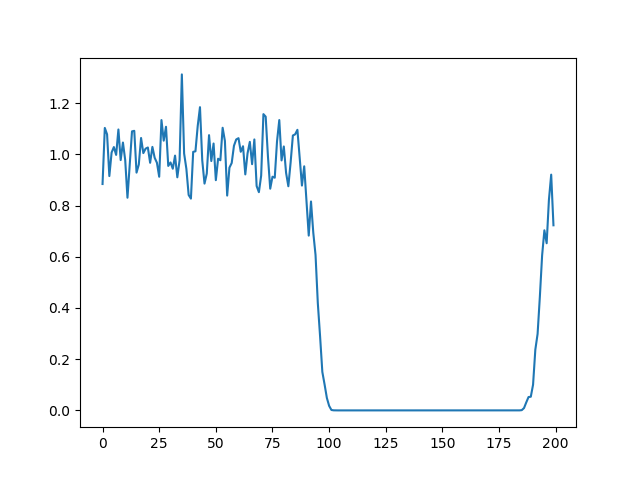
\includegraphics[scale=0.4]{water_density_profile}
\caption{Density of water component across 200 bins in the interface normal direction.}
\end{figure}

We then fit to the error function profile as described in Patel et. al (2006), and obtain the following parameters: $\rho_W = 0.997, h_W = 94.212, w_c = 1.87 Angstroms$, which is in good agreement with previous simulations and experiments.  A plot of the fit is shown below: 

\begin{figure}[H]
\centering
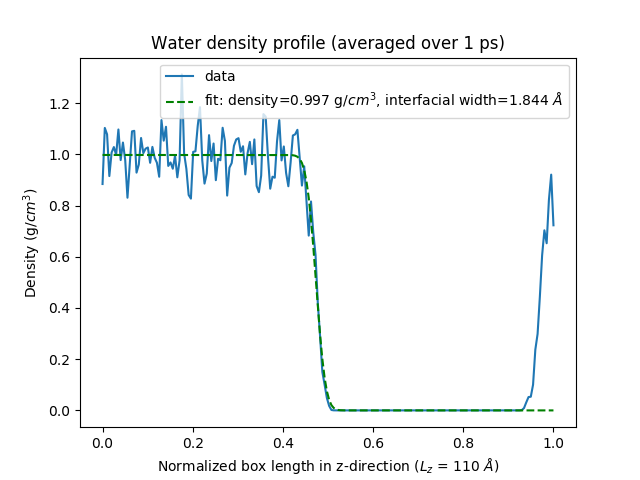
\includegraphics[scale=0.4]{water_density_profile_fit}
\caption{Density of water component across 200 bins in the interface normal direction.}
\end{figure}

\end{enumerate}

\subsection{4/5/2018}

\begin{enumerate}
\item I checked that hexane.in.settings, which contains the intramolecular mixing rules for TAFFI hexane, exhibits Waldman-Hagler mixing:

\begin{align}
\begin{split}
\epsilon_{ij} = 2\sqrt{\epsilon_i\epsilon_j}\left(\frac{\sigma_i^3\dot\sigma_j^3}{\sigma_i^6 + \sigma_j^6}\right)\\
\sigma_{ij} = \left(\frac{\sigma_i^6 + \sigma_j^6}{2}\right)^{\frac{1}{6}}
\end{split}
\end{align}

\item I added the following functionality to interface.py: collecting densities for both water and hexane, and deciding standard versus waldman-hagler mixing, number of equilibration and production steps, the output filenames.  Below is a preliminary figure of combined density profiles taken from just 2000 simulation steps: 

\begin{figure}[H]
\centering
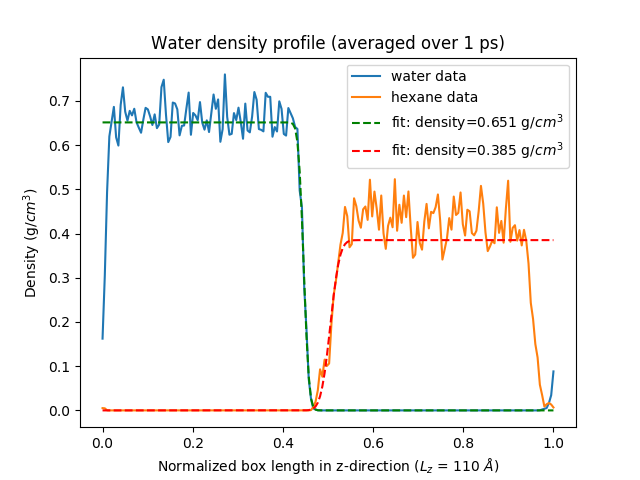
\includegraphics[scale=0.4]{double_profile_test}
\caption{Double density profile test.}
\end{figure}

\item I am now running : DASH simulation of 500 TAFFI hexane, 3650 TIP4P/F water, standard mixing, NPT Andersen/Berendsen at T = 298.15 K and P = 1.0 atm, 300,000 timesteps of length 0.5 fs equilibration followed by 100000 production steps of length 0.5 fs, NPT pre-equilibration of each slab at 298.15 K and same P.  Cutoff = 12.0, Ewald summation.  Classical simulation, no path integrals.  During production run, computing density of water in 200 parallel slabs along the z-direction every 100 simulation steps.  

\item For waldman, I am now running the same as above except waldman mixing, 400,000 equilibration steps only 1000 production, no density calculation.  

\end{enumerate}

\subsection{4/9/2018}

\begin{enumerate}
\item Finished the following run: DASH simulation of 500 TAFFI hexane, 3650 TIP4P/F water, standard mixing, NPT Andersen/Berendsen at T = 298.15 K and P = 1.0 atm, 300,000 timesteps of length 0.5 fs equilibration followed by 100000 production steps of length 0.5 fs, NPT pre-equilibration of each slab at 298.15 K and same P.  Cutoff = 12.0, Ewald summation.  Classical simulation, no path integrals.  During production run, computing density of water in 200 parallel slabs along the z-direction every 100 simulation steps.

\item Problem: After step 300400, i.e. after 400 production steps, the program quits with a "segmentation fault" error.  

\item Although there were only three datapoints, nevertheless it is worth pointing out that the system was able to collect both water and hexane densities.  Using the density profile analysis script, we obtain the following plot of the profile over the first 400 production steps: 

\begin{figure}[H]
\centering
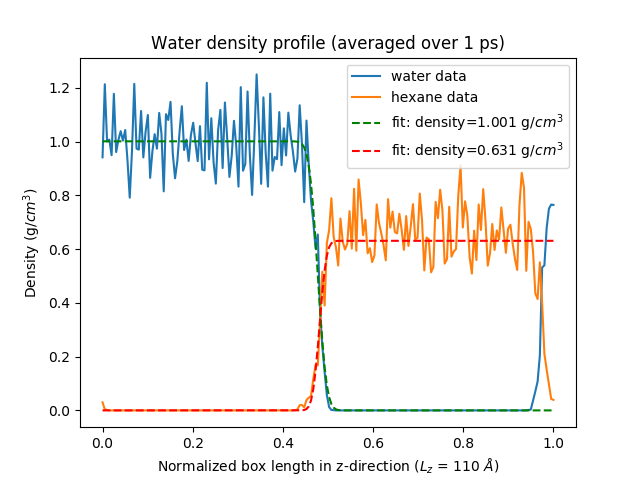
\includegraphics[scale=0.4]{double_profile}
\caption{Double density profile after 400 production steps as described above.  Densities and profiles look reasonable.}
\end{figure}

\item Also ran the same as above excep using waldman mixing, 400,000 equilibration steps only 1000 production, no density calculation.  Here is a plot after the whole simulation:

\begin{figure}[H]
\centering
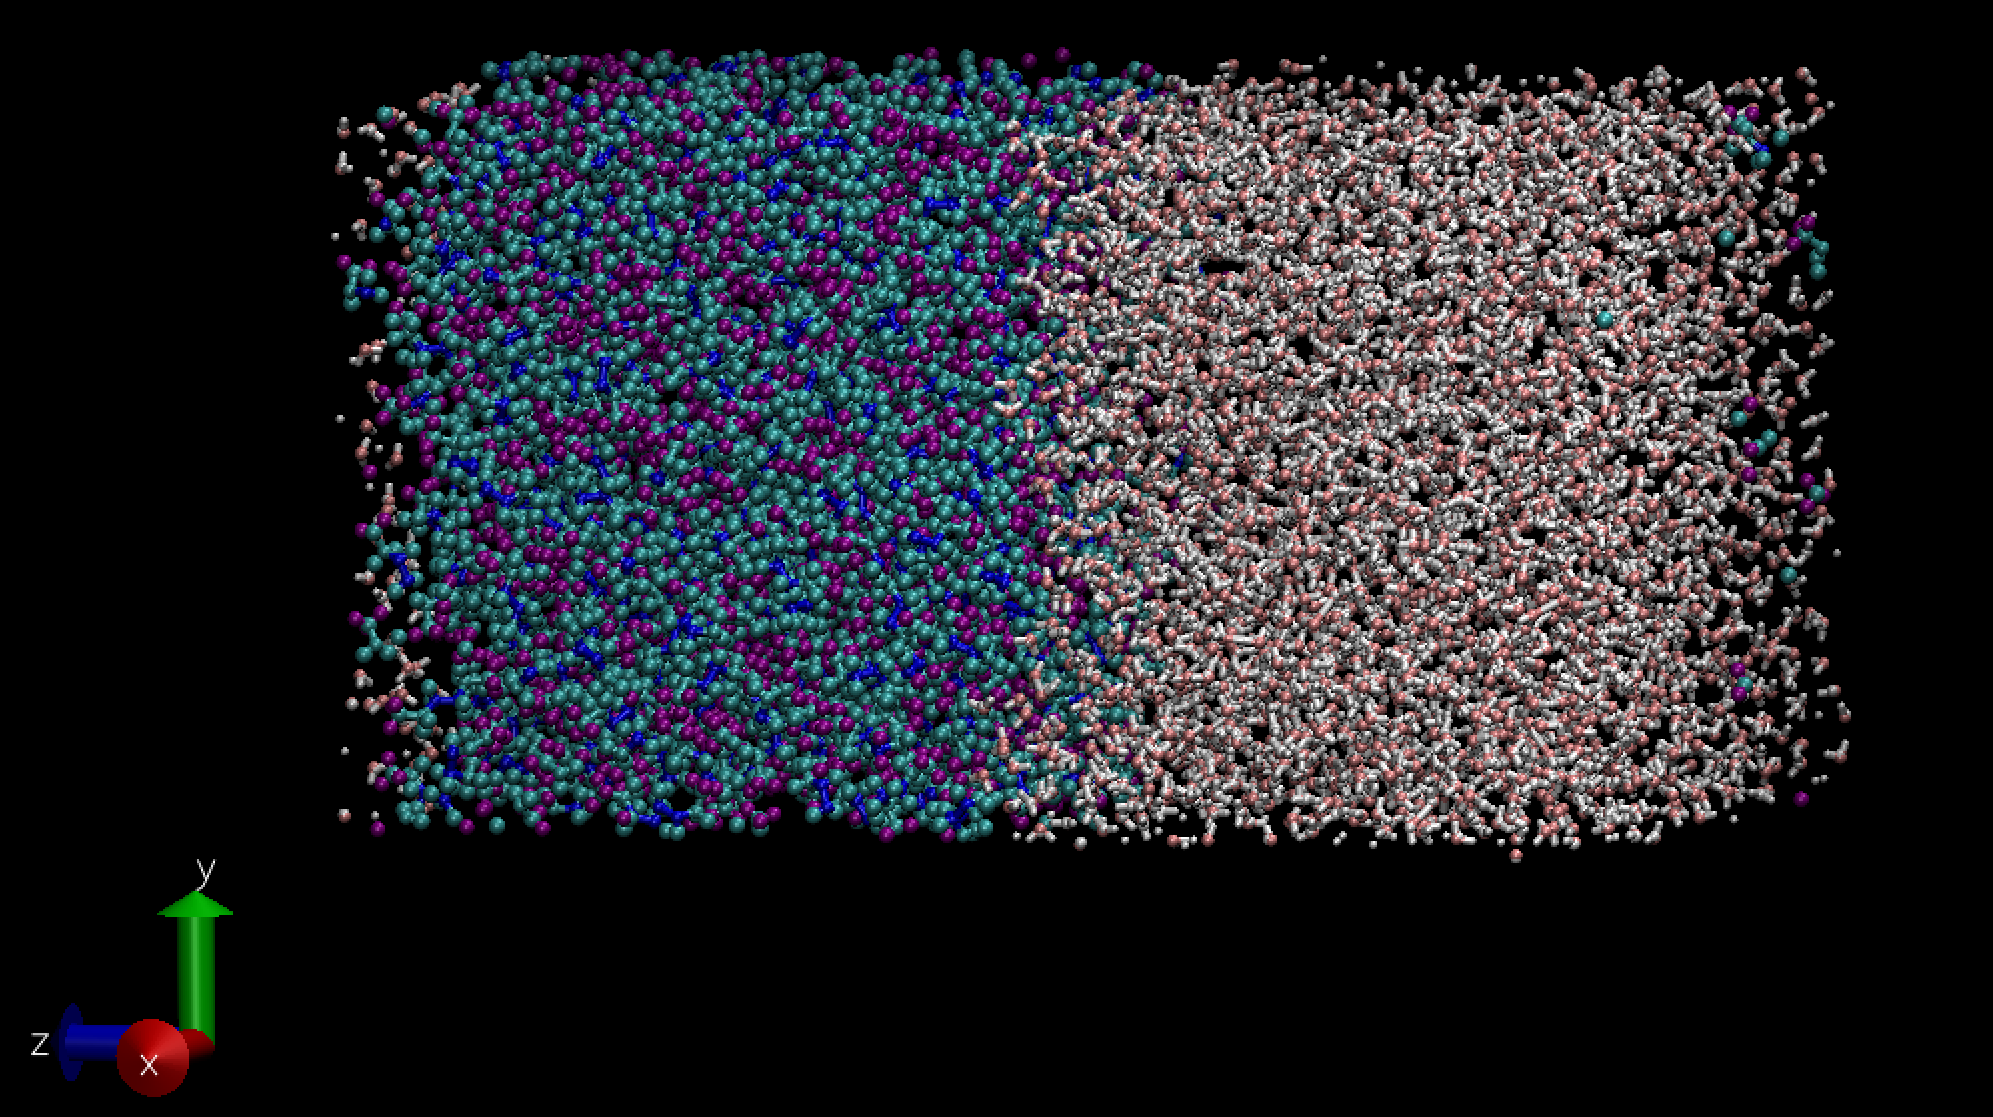
\includegraphics[scale=0.4]{waldman_pic}
\caption{Final snapshot of simulation as described above with Waldman-Hagler mixing.  Looks reasonable.}
\end{figure}

\item From now on we will use W-H mixing.  However, there is still the problem of segmentation fault.  So, we will run three tests o try to discover the origin of this error:
\item Test 1: Run a program that does 300000 pre-equilibration steps and 300000 production steps, no density calculation, see if an error occurs.
\item Test 2: Run a program that does 600000 total pre-equilibration steps and only 1 production step (basically zero production), see if an error occurs, no density calculation.
\item Test 3: Run a program that does 300000 pre-equilibration steps and 300000 production steps, computing the density the whole time. 
\item Test 4: Run a program that does 600000 pre-equilibration steps and 300000 production steps, computing density the whole time.   

\item For the sake of not repeating information, until I note otherwise, all DASH interfacial simulations have the following properties: 500 TAFFI hexane, 3650 TIP4P/F water, waldman-hagler mixing, NPT Andersen/Berendsen at T = 298.15 K and P = 1.0 atm, timestep 0.5 fs, NPT pre-equilibration of each slab at 298.15 K and same P.  Cutoff = 12.0, Ewald summation.  Classical simulation, no path integrals. 

\item Test 1: Running it now.  
\item Test 2: Running now.  
\item Test 3: Running now.  

\item We also want to test density as a function of temperature for the pure hexane and pure water systems.  Let's start with hexane.  In in.webb\_hexane.py, added a final line that computes the standard deviation as well as mean of list of densities.  Mean and sd are computed for the last 500 recordings of density.  Ran lammps\_replicator script to produce input.txt script of initial 500 molecule hexane lattice.  Running DASH system with 500 TAFFI molecules, W-H mixing, NPT Andersen/Berendsen at T = 298.15 K and P = 1.0 atm, timestep of 1 fs, cutoff = 10, 2,000,000 steps.  Density is calculated every 100 steps, and the mean and sd calculations below represent the last 500 recordings, or 50,000 steps.  

\item T = 298.15 K, $\rho = 0.65166 g/ml$, $\sigma = 0.0004788 g/ml$, expt: 0.65478 $g/ml$ on NIST Chemistry Webbook at P = 1.0 atm.  So, the density is off by -0.476\%.  
\item T = 320 K, $\rho = 0.62475 g/ml$, $\sigma = 0.00072859 g/ml$, expt: 0.63434 $g/ml$.  So, the density is off by -1.5118\%.  
\item T = 270 K, $\rho = 0.68196 g/ml$, $\sigma = 0.000927 g/ml$, expt: 0.68025 $g/ml$.  So, the density is off by +0.25\%.  


\item Now we will move onto water.  Created a new file in.tip4pF\_dens.py, in which I added the same mean and sd calculations as above.  Time step 0.5 fs, 2,000,000 steps, initial density of 0.997, 3650 molecules, cutoff = 9.0.  Running this now.  

\item T = 298.15K, $\rho = 0.98919 g/ml$, $\sigma = 0.00116 g/ml$, https://webbook.nist.gov/cgi/fluid.cgi?ID=C7732185\&Action=Page expt: 0.99705 $g/ml$ at P = 1.0 atm.  So, the density is off by -\%0.00788.   
\item T = 270K, $\rho = 0.988 g/ml$, $\sigma = 0.001555 g/ml$, but this is below freezing??
\item T = 300 K, $\rho = 0.9877 g/ml$, $\sigma = 0.0034977$, expt: 0.99656.  So, the density is off by -0.00889 \%
\item T = 320 K, $\rho = 0.98157 g/ml$, $\sigma = 0.0022$, expt: 0.989.  So, the density is off by -0.0075\%.  


\item RESULT: Test 1 ran perfectly fine.  300,000 pre-equilibration, 300,000 production, no density calculation, no segmentation fault!  
\item RESULT: Test 2 ran perfectly fine.  600,000 pre-equilibration steps, 1 production step, 1 production step, no density calculation, no segmentation fault!
\item Running test 3 still.  

\item Note: the units for mass in DASH are amu, and the units for distance are Angstroms.  So, we use the conversion factor $\frac{1}{0.6022}$ to convert this to $g/ml$.  

\item Test 4: Same as test 3, but density calc is only every 1000 turns instead of every 100 turns.  This is the REAL test 4, not as described above.    

\item Created an interface\_hexane\_restart.py file that spits out a hexane\_interface\_restart.txt file, and tried constructing an interface\_restart.py file, but resulted in green's function errors.  It creates an initial configuration that looks fine but does not integrate the system.  

 
\item Change densities.txt file names in interface.py!  
\end{enumerate}

\subsection{4/12/2018}
\begin{enumerate}
\item RESULT: Test 3, program stopped after 107300, 35.77 \% done, Fatal Python error: GC object already tracked.  /tmp/slurmd/job44973736/slurm\_script: line 30: 12701 Aborted.  Computing densities every 100 steps.  
\item RESULT: Test 4, program stopped after 112300, 37.43 \% done, computing density every 1000 steps.  Segmentation fault error.  
\item Ok, in order to diagnose this problem, let's run more tests.  

\item Test 5: 300,000 preequilibration steps, 300,000 production steps, density profile function computing density every 1000 steps is there but not activated in the sbatch script.
\item Test 6: Same as test 5, except actually computing the density as usual every 1000 steps.
\item Test 7: Same as above, except the density profile does not actually comput anything.
\item Test 8: Same, except density function only active up to the loop.
\item Test 9: Same, except density function only active up to the first write file command.  
\item Test 10: Same, except density only active until last write file.
\item Hopefully, these tests will dig into the details of excactly where the issue is arising.  
\item Sent a message to Brian about this issue, and got a response saying I should try "In your PythonOperation() constructor in the python script, did you set synchronous=True?  If not, I would try that.  The default behavior is asynchronous."  So, before running all of these tests, I will try this first!
\item In the file for test 5, called interface\_test5.py, I made this change to PythonOperation().  Let's try this now. 
\item It appears to be working.  Modified the original interface.py to reflect this, as well as customizing filename for the density files.  Currently running DASH simulation of the interface using 400,000 preequilibration steps, followed by 300,000 production steps during which density profiles are measured every 100 steps.   
\end{enumerate}

\subsection{4/17/2018}

\begin{enumerate}
\item What we really need is to do post-production.  So, for the successful run above, we are just going to take the trajectory file and analyze that.  In this case, the file is interface-dens.xyz.  
\end{enumerate}

\subsection{4/18/2018}

\begin{enumerate}
\item Here are the results from our analysis: 

\subitem Bulk water density: 0.999247086118 $g/cm^3$
\subitem Bulk hexane density: 0.674945918949 $g/cm^3$
\subitem Intrinsic width: 0.712788562077 Angstroms
\subitem Water thermal width: 1.89474070104 Angstroms
\subitem Hexane thermal width: 1.85287262473 Angstroms

\begin{figure}[H]
\centering
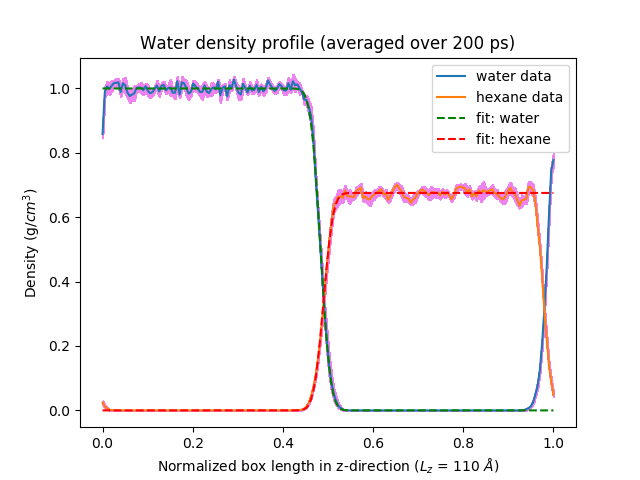
\includegraphics[scale=0.4]{double_profile_with_errors}
\end{figure}

\item Based on inspection, the average box length in the z-direction is assumed to be 110.0 Angstroms.  Also based on visual inspection of the profiles, the bulk region for water is determined to be 0.1 < z < 0.4, while the bulk region for hexane is 0.6 < z < 0.85.  The bulk densities for each are computed in those respective regions.  The curve fits for error function profiles, described in Patel and Brooks 2006, are fit using scipy curve\_fit function, where the bulk densities are specified but not the Gibbs dividing surfaces or the thermal width.  The widths are left to be separate.  The fits are done only in the interfacial region of the data, which is determined by inspection to be 0.4 < z < 0.6.  The standard error measurements are performed by dividing the 200 ps data into 5 blocks, and finding the SE of the mean across all 200 bins over which the averaeg profiles are computed.  The result of the SE is shaded in pink for each profile.  

\item We will now run a simulation that computes 300,000 equilibration steps and 1,000,000 ps production.  The system will be NPT in equilibration, but then immediately fixed to NVT in production.  No density calculation.  Although it would be optimal to calculate the average box length after equilibration and then set V to that box length, for now we will skip that step.  NVT is to ensure that we have fixed bins over which to compute density profiles.  The python script will be named interface\_NVT.py.  


\end{enumerate}

\section{4/22/2018}

\begin{enumerate}
\item Wrote python script, molecular\_orientation\_postproduction.py that computes $S_{zz}$ in 200 slabs, and then orientation\_profile\_analysis.py that averages and plots them.  Here is the result for water:

\begin{figure}[H]
\centering
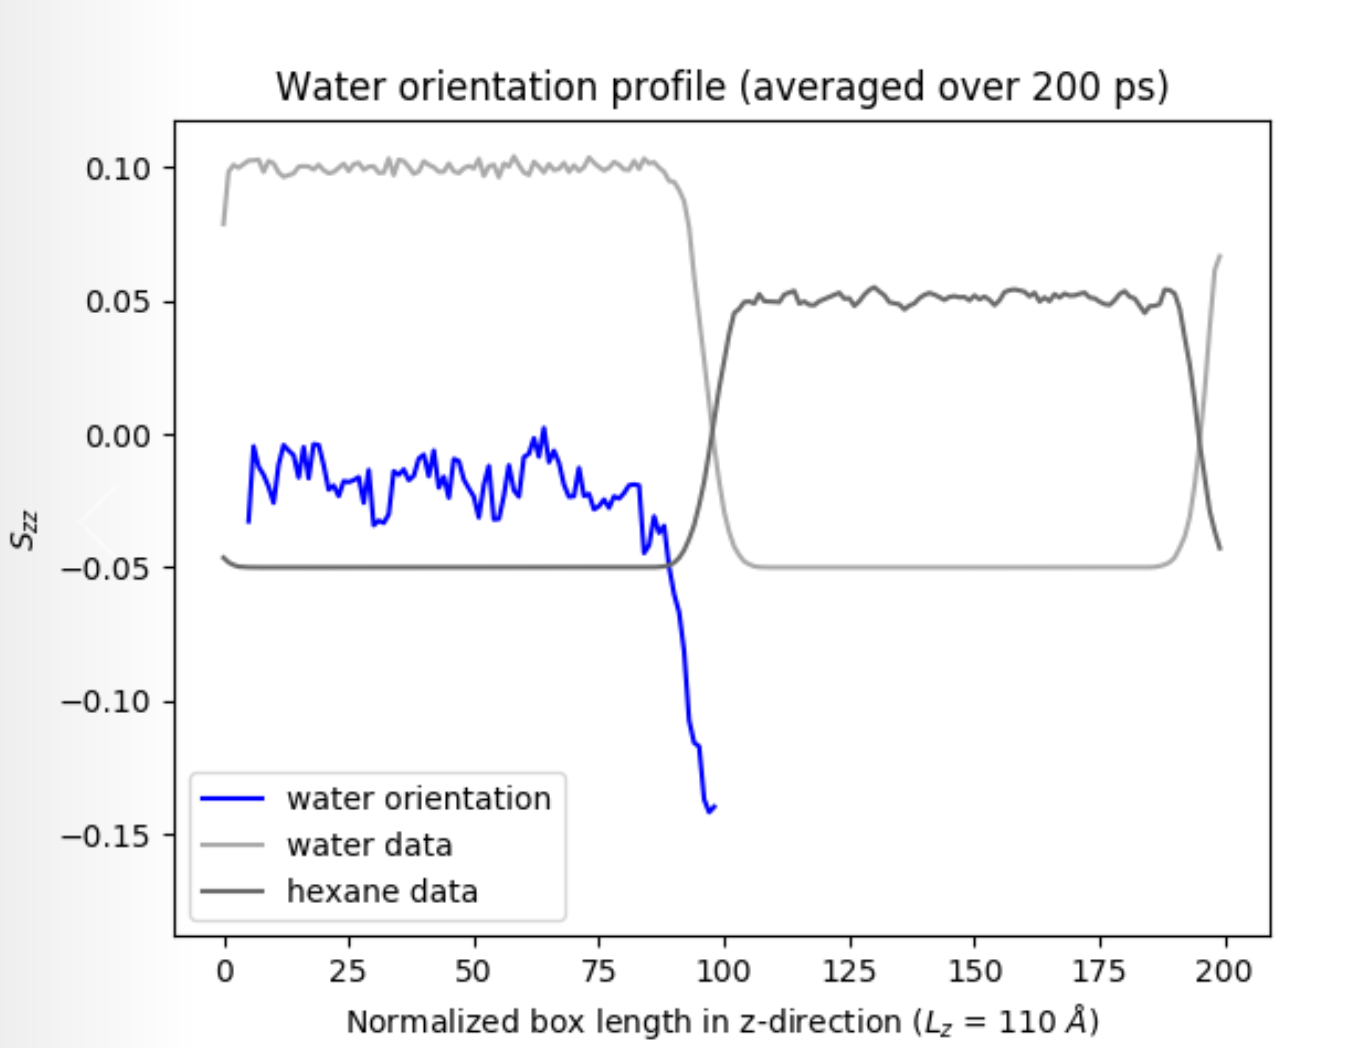
\includegraphics[scale=0.4]{water_orientation}
\end{figure}

which compares favorably to one of the models discussed in Patel and Brooks (2006):
\begin{figure}[H]
\centering
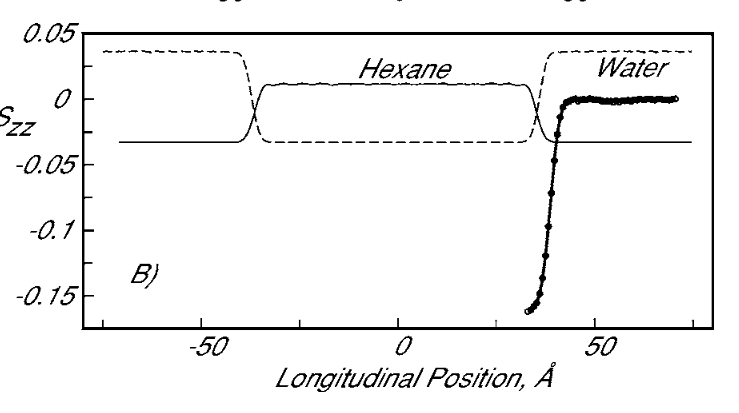
\includegraphics[scale=0.4]{patel_water_orientation}
\end{figure}

These results indicate that water dipole moment is isotropic in the bulk, but orients preferentially along the interface in the interfacial region.  For hexane, we see:

\begin{figure}[H]
\centering
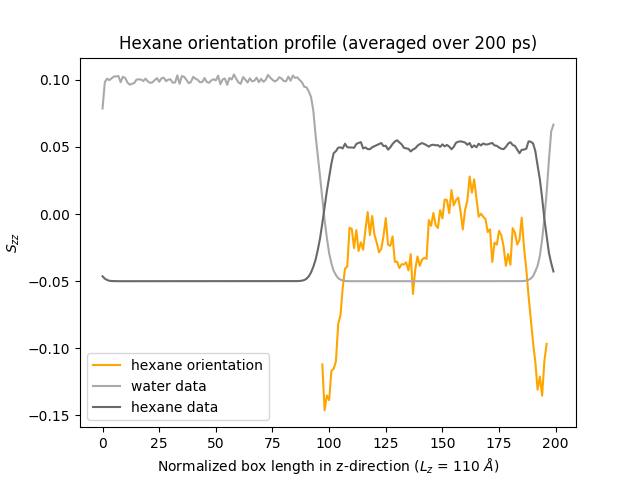
\includegraphics[scale=0.4]{orientation_hexane}
\end{figure}

This also matches with Patel:

\begin{figure}[H]
\centering
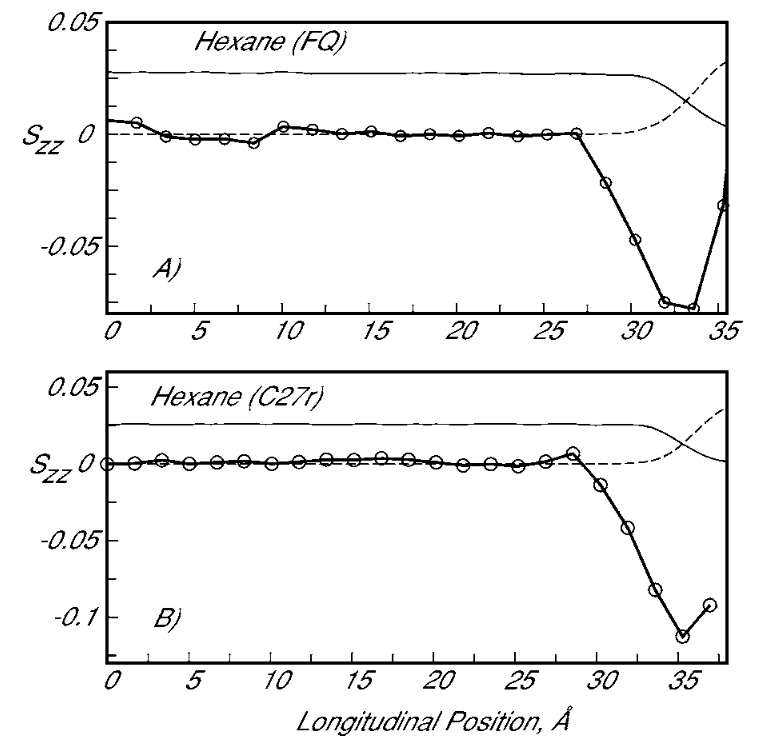
\includegraphics[scale=0.4]{patel_hexane_orientation}
\end{figure}



\end{enumerate}

\subsection{4/23/2018}

\begin{enumerate}
\item Compiled latest version of DASH, placed in /home/swansonk1/NEW\_DASH.  Copied the water.py from utils.py in OLD\_DASH.  Everything seems to run smoothly, including restart files!  
\item So now, we will run the file interface\_new.py, which has the link to new dash.  We will do 400,000 steps (i.e. 200 ps) of equilibration.  Prints restart file every 10,000 steps.  Run file is run\_new.sh.    
\end{enumerate}

\section{4/24/2018}

\begin{enumerate}
\item Trajectory data for interface\_NVT.py is contained in interface-NVT.xyz.  
\item The first thing we want to do is to construct a production run dataset that has path integrals.  We used interface\_new.py and run\_new.sh to perform a 400,000 step (i.e. 200 ps) equilibration in NPT using the standard parameters.  Now, we will restart that simulation, except we will use path integral beads.  As proof of concept, we will start with just a few, say 16 beads.  
\end{enumerate}













\end{document}

%%%%%%%%%%%%%%%%%%%%%%%%%%%%%%%%%%%%%%%%%%%%%%%%%%%%%%%%%%%%%%%%%%%%%%%%%%%%%%%%%%%%%%%%%%%%%%%%%%%%%%%%%%%%%%%%%%%%%%%%%%%%%%